\documentclass{article}
\usepackage[utf8]{inputenc}
\ProvidesPackage{lindrew}[2020/05/09] % with great amounts of help from Jason Chen

\newif\iflinserif \linseriffalse % by default, uses cmbright sans serif font.
\newif\iflinclass \linclasstrue % by default, numbers all theorems/definitions from 1 to N w/o regard for section
\newif\iflinindent \linindenttrue % by default, does do paragraph indent
\newif\iflinheader \linheadertrue % by default, no header

\DeclareOption{serif}{\linseriftrue}  % if you don't like the font
\DeclareOption{formal}{\linclassfalse} % if you want a document where theorems in section 1 are "theorem 1.x", etc.
\DeclareOption{noindent}{\linindentfalse}
\DeclareOption{header}{\linheadertrue}

\ProcessOptions*

\iflinserif\else
    \usepackage{cmbright}
\fi

\iflinindent
\else
    \setlength{\parindent}{0pt}
\fi

\iflinheader
    \usepackage[includehead,includefoot, heightrounded,  left=0.8in, top=1.6cm, bottom=2.4cm, right=0.8in]{geometry}
    \usepackage{fancyhdr}
    \pagestyle{fancy}
    \rhead{\textbf{Mauricio Barba da Costa}} % change name as necessary
\else
    \usepackage[left=0.8in, top=1.6cm, bottom=2.4cm, right=0.8in]{geometry}
\fi

\usepackage{amsmath, amssymb, amsthm} % standard
\usepackage[svgnames, dvipsnames, usenames]{xcolor}
\usepackage[colorlinks]{hyperref} % inserting links - copied from Jason
\PassOptionsToPackage{colorlinks}{hyperref}
\hypersetup{urlcolor = RedViolet, linkcolor = RoyalBlue, citecolor = ForestGreen}
\urlstyle{same}

\usepackage[capitalize]{cleveref} % for cross-referencing theorems, etc.
\usepackage{graphicx} % for putting pictures
\usepackage[T1]{fontenc} % for accents, etc.
\usepackage{verbatim} % for commenting out sections of text
\usepackage[nodisplayskipstretch, onehalfspacing]{setspace} % 1.5 spacing
\usepackage{tikz, tikz-cd, pgfplots} % for drawing pictures
\usepackage[style=numeric, sorting=none]{biblatex} % citations
\renewbibmacro{in:}{} % remove "In:" in the bibliography

\newcommand{\vocab}[1]{\textbf{\color{blue!90}\boldmath #1}}
\newcommand{\paren}[1]{\left(#1\right)}
\newcommand{\pnorm}[1]{\left|\left|#1\right|\right|}
\newcommand{\floor}[1]{\left\lfloor#1\right\rfloor}

% Fixes itemize
\usepackage{enumitem}
\setlist{itemsep = 0.2em, topsep = 0.4em}
\renewcommand\labelitemi{\raisebox{0.15em}{\tiny$\bullet$}}

% Changes size of section headers
\usepackage{titlesec}
\titleformat*{\section}{\LARGE\bfseries\sffamily}
\titleformat{\subsection}{\Large\bfseries\sffamily}{\thesubsection}{0.4cm}{}

% Blackboard bold
\newcommand{\Aff}{\mathbb{A}}
\newcommand{\C}{\mathbb{C}}
\newcommand{\F}{\mathbb{F}}
\newcommand{\G}{\mathbb{G}}
\newcommand{\bbH}{\mathbb{H}}
\newcommand{\N}{\mathbb{N}}
\newcommand{\PP}{\mathbb{P}}
\newcommand{\Q}{\mathbb{Q}}
\newcommand{\R}{\mathbb{R}}
\newcommand{\Sphere}{\mathbb{S}}
\newcommand{\Z}{\mathbb{Z}}
\newcommand{\Qbar}{{\overline{\Q}}}
\newcommand{\Zhat}{{\widehat{\Z}}}
\newcommand{\Zbar}{{\overline{\Z}}}
\newcommand{\kbar}{{\overline{k}}}
\newcommand{\Kbar}{{\overline{K}}}
\newcommand{\Fbar}{{\overline{\F}}}

\newcommand{\boldmu}{\bm{\mu}}
\newcommand{\boldalpha}{\bm{\alpha}}

\newcommand{\ii}{\mathbf{i}}
\newcommand{\jj}{\mathbf{j}}
\newcommand{\kk}{\mathbf{k}}

\newcommand{\pp}{\mathfrak{p}}
\newcommand{\mm}{\mathfrak{m}}

% mathcal characters
\newcommand{\calA}{\mathcal{A}}
\newcommand{\calB}{\mathcal{B}}
\newcommand{\calC}{\mathcal{C}}
\newcommand{\calD}{\mathcal{D}}
\newcommand{\calE}{\mathcal{E}}
\newcommand{\calF}{\mathcal{F}}
\newcommand{\calG}{\mathcal{G}}
\newcommand{\calH}{\mathcal{H}}
\newcommand{\calI}{\mathcal{I}}
\newcommand{\calJ}{\mathcal{J}}
\newcommand{\calK}{\mathcal{K}}
\newcommand{\calL}{\mathcal{L}}
\newcommand{\calM}{\mathcal{M}}
\newcommand{\calN}{\mathcal{N}}
\newcommand{\calO}{\mathcal{O}}
\newcommand{\calP}{\mathcal{P}}
\newcommand{\calQ}{\mathcal{Q}}
\newcommand{\calR}{\mathcal{R}}
\newcommand{\calS}{\mathcal{S}}
\newcommand{\calT}{\mathcal{T}}
\newcommand{\calU}{\mathcal{U}}
\newcommand{\calV}{\mathcal{V}}
\newcommand{\calW}{\mathcal{W}}
\newcommand{\calX}{\mathcal{X}}
\newcommand{\calY}{\mathcal{Y}}
\newcommand{\calZ}{\mathcal{Z}}

\newcommand{\CC}{\mathscr{C}}
\newcommand{\FF}{\mathscr{F}}
\newcommand{\GG}{\mathscr{G}}
\newcommand{\scriptH}{\mathscr{H}}
\newcommand{\II}{\mathscr{I}}
\newcommand{\JJ}{\mathscr{J}}
\newcommand{\KK}{\mathscr{K}}
\newcommand{\LL}{\mathscr{L}}
\newcommand{\OO}{\mathscr{O}}
\newcommand{\XX}{\mathscr{X}}
\newcommand{\ZZ}{\mathscr{Z}}

% various math expressions that shouldn't be italicized
\DeclareMathOperator{\cis}{cis}
\DeclareMathOperator{\var}{var}
\DeclareMathOperator{\Var}{Var}
\DeclareMathOperator{\Cov}{Cov}
\DeclareMathOperator*{\lcm}{lcm}
\DeclareMathOperator{\ord}{ord}
\DeclareMathOperator{\Ker}{Ker}
\DeclareMathOperator{\Bin}{Bin}
\DeclareMathOperator{\res}{res}
\DeclareMathOperator{\rad}{rad}
\DeclareMathOperator{\Spec}{Spec}

\newcommand{\Cech}{\v{C}ech}
\newcommand{\del}{\partial}
\newcommand{\directsum}{\oplus} % binary direct sum
\newcommand{\Directsum}{\bigoplus} % direct sum of a collection
\newcommand{\injects}{\hookrightarrow}
\newcommand{\intersect}{\cap} % binary intersection
\newcommand{\Intersection}{\bigcap} % intersection of a collection
\newcommand{\isom}{\simeq}
\newcommand{\HH}{{\operatorname{H}}}
\newcommand{\HHcech}{{\check{\HH}}}
\newcommand{\HHat}{{\hat{\HH}}}
\newcommand{\notdiv}{\nmid}
\newcommand{\surjects}{\twoheadrightarrow}
\newcommand{\tensor}{\otimes} % binary tensor product
\newcommand{\Tensor}{\bigotimes} % tensor product of a collection
\newcommand{\To}{\longrightarrow}
\newcommand{\union}{\cup} % binary union
\newcommand{\Union}{\bigcup} % union of a collection

% can't use DeclareMathOperator because already defined
\renewcommand{\Re}{\operatorname{Re}}
\renewcommand{\Im}{\operatorname{Im}}
\renewcommand{\mod}[1]{\ \text{mod}\ #1}

% other convenient abbreviations
\newcommand{\eps}{\varepsilon}
\DeclareMathOperator{\indep}{\perp\!\!\!\perp}

% Mau's new commands
\newcommand{\f}[2]{\frac{#1}{#2}}
\newcommand{\ra}[1][]{\xrightarrow{#1}}
\DeclareMathOperator{\inn}{inn}
\DeclareMathOperator{\id}{id}
\DeclareMathOperator{\im}{im}
\DeclareMathOperator{\Span}{Span}
\DeclareMathOperator{\tr}{tr}
\DeclareMathOperator{\Stab}{Stab}

% theorem boxes
\usepackage{thmtools}
\usepackage[framemethod = TikZ]{mdframed}
\usepackage{silence} % for suppressing warnings
\WarningFilter{mdframed}{You got a bad break}

\mdfsetup{
	linewidth = 0.3mm,
	innertopmargin = 2mm,
	innerbottommargin = 3.5mm,
	innerleftmargin = 3mm,
	innerrightmargin = 3mm
} % adjusts boundaries of boxes

\newcommand{\thmboxstyle}[4]{
	\mdfdefinestyle{#2}{
		linecolor = #3,
		backgroundcolor = #4,
		nobreak = true
	}
	\declaretheoremstyle[
		headfont = \sffamily\bfseries\color{#3},
		mdframed = {style = #2},
		headpunct = {\\[0.4pt]},
		postheadspace = {0pt},
	]{#1}
}

% four different colors of boxes

\thmboxstyle{defbox}{mdredbox}{red}{orange!5}
\thmboxstyle{thmbox}{mdbluebox}{blue!90!red}{cyan!4}
\thmboxstyle{exbox}{mdgreenbox}{green!70!black}{teal!4}
\thmboxstyle{notebox}{mdorangebox}{orange!50!brown}{yellow!5!olive!5}

\iflinclass
    \declaretheorem[style = thmbox, name = Theorem]{theorem}
\else
    \declaretheorem[style = thmbox, name = Theorem, numberwithin = section]{theorem}
\fi

\declaretheorem[style = thmbox, name = Lemma, sibling = theorem]{lemma}
\declaretheorem[style = thmbox, name = Proposition, sibling = theorem]{proposition}
\declaretheorem[style = thmbox, name = Corollary, sibling = theorem]{corollary}
\declaretheorem[style = thmbox, name = Conjecture, sibling = theorem]{conjecture}

\declaretheorem[style = thmbox, name = Theorem, numbered = no]{theorem*}
\declaretheorem[style = thmbox, name = Lemma, numbered = no]{lemma*}
\declaretheorem[style = thmbox, name = Proposition, numbered = no]{proposition*}
\declaretheorem[style = thmbox, name = Corollary, numbered = no]{corollary*}
\declaretheorem[style = thmbox, name = Conjecture, numbered = no]{conjecture*}

\declaretheorem[style = defbox, name = Definition, sibling = theorem]{definition}
\declaretheorem[style = defbox, name = Definition, numbered = no]{definition*}

\declaretheorem[style = exbox, name = Example, sibling = theorem]{example}
\declaretheorem[style = exbox, name = Example, numbered = no]{example*}

\declaretheorem[style = notebox, name = Fact, sibling = theorem]{fact}
\declaretheorem[style = notebox, name = Fact, numbered = no]{fact*}
\declaretheorem[style = notebox, name = Problem, sibling = theorem]{problem}
\declaretheorem[style = notebox, name = Problem, numbered = no]{problem*}

\declaretheorem[style = plain, name = Question, sibling = theorem]{question}
\declaretheorem[style = plain, name = Question, numbered = no]{question*}

\declaretheorem[style = plain, name = Claim, sibling = theorem]{claim}
\declaretheorem[style = plain, name = Claim, numbered = no]{claim*}

\declaretheorem[style=plain, name=Remark, sibling=theorem]{remark}
\declaretheorem[style=plain, name=Remark, numbered=no]{remark*}

% Makes title bold
\makeatletter
\patchcmd{\@maketitle}{\LARGE}{\LARGE\bfseries}{}{}
\makeatother
\title{Algebra notes}
\author{Mauricio Barba da Costa}

\begin{document}

\maketitle

\section{September 11, 2020}
Group theorists somethings denote $H\leq G$ if $H$ is a subgroup of G (not just a subset). This is what we covered last time.
\begin{definition}
    The index of $H$ in G is denoted $(G:H):=$ the number of left cosets of $H$ in $G$.
\end{definition}
\begin{theorem}[The counting formula]
    $|G|=|H|(G:H)$
\end{theorem}
\begin{corollary}[Lagrange's theorem]
If $G$ is finite, then $|H|$ divides $|G|$.
\end{corollary}
\begin{corollary}
If $|G|$ is prime then $G\cong C_p$
\end{corollary}
\hrule
\begin{corollary}[Corollary to the counting formula]
If $\phi:G\ra{} G'$ then $|G|=|\ker\phi||\Im\phi|$
\end{corollary}
\begin{proof}
Let $K=\ker\phi$. The counting formula says that $|G|=|K|(G:K)=|\ker\phi||\Im\phi|$ since the number of cosets of $K$ is in bijection with $\Im\phi$.
\end{proof}
\begin{definition}
    Let $G$ be a group and $H$ a subgroup. $H$ is normal in $G$ if and only if for all $g\in G$ and $g\in H$, $ghg^{-1}\in H$.
\end{definition}
Equivalently, for all $g\in G$, $gHg^{-1}\subseteq H$. In particular, $gHg^{-1}=H$. If $gHg^{-1}\subseteq H$ and $g^{-1}Hg\subseteq H$, multiplying both sides gives $H\subseteq gHg^{-1}$. Thus $gHg^{-1}=H$. For all $g\in G$ $\inn_g(H)=H$. For all $g\in G$, $gH=Hg$.

Not all subgroups are normal but we can run through a bunch of examples:
\begin{example}
The kernel of any homomorphism is normal. This is the reason normal subgroups are important
\end{example}
\begin{proof}
Suppose there exists $\phi:G\ra{}G'$ and $H=\ker\phi$. Let $g\in G$ and $h\in H$. Then $\phi(ghg^{-1}=\phi(g)\phi(h)\phi(g)^{-1}=\phi(g)\phi(g)^{-1}=\id$. Hence, the kernel is normal.
\end{proof}
\begin{example}
If $G$ is abelian, any subgroup $H$ is normal
\end{example}
\begin{proposition}
Any subgroup of index 2 is normal.
\end{proposition}
\begin{proof}
Let $H$ is a subgroup of $G$ of index 2. The two left cosets is $H$ are $H$ and $gH$ where $g\notin H$. The two right cosets are $H$ and $Hg$ where $g\notin H$. Thus the left and right cosets are the same
\end{proof}
\begin{example}
The center $Z(G)$ of a group $G$ is a normal subgroup. This is the set $\{z\in G:zg=gz\forall g\in G\}$.
\end{example}
\begin{proof}[An alternative proof of the fact that $Z(G)$ is normal]
If you have an isomorphism $\phi:G\ra{}G'$ maps the center of $G$ to the center of $G'$. Take $\phi$ to be $\inn_g:G\ra{}G$. You get $\inn_g(Z)=Z$. This holds for every $g$.
\end{proof}
\begin{fact}
Any subgroup that can be described without naming specific elements is a normal subgroup. Such a description respects any isomorphism and in particular the inner automorphisms.
\end{fact}
\begin{example}
The subgroup of $G$ generated by all elements of order 2 is automatically normal because of the above fact.
\end{example}
\begin{example}[Subgroups of $S_3$]
$S_3=\{1,(1 2), (1 3), (2 3), (1 2 3), (1 3 2)\}$. You can take the cyclic subgroups $<(1 2)>, <(13)>, <(23)>, <(123)>$. I claim that these are all the subgroups. If you have any other subgroup $H$, it must contain $<(12)>$ and it is contained in $S_3$. Thus $|H||6$ and $2||H|$ so $H$ is either one of the cyclic subgroups or the entire group.
\end{example}
Subgroup lattices are a thing. At the top but the group $G$. At the bottom put the trivial group. Make rows between the group and the trivial group with the divisors of $|G|$. If a subgroup has order $n$ put it in row $n$. If a subgroup is a subgroup of another put a line between the two.
\begin{proposition}
Let $\phi:G\ra{}G'$ be a homomorphism. If $H\leq G$ then $\phi(H)\leq G'$. If $H$ is a normal subgroup of $G$ and $\phi$ is surjective then $\phi(H)$ is a normal subgroup of $G'$.
\end{proposition}
\begin{proposition}
If $H'\leq G'$ then $\phi^{-1}(H')\leq G$. If $H'$ is a normal subgroup of $G'$ then $\phi(H')$ is a normal subgroup of $G$.
\end{proposition}
\begin{proof}
Suppose that $g\in G$ and $h\in \phi^{-1}(H')$. Then $\phi(h)\in H'$ so $\phi(ghg^{-1})=\phi(g)\phi(h)\phi(g)^{-1}\in H'$ since $H'$ is normal in $G'$. Thus $\phi^{-1}(H')$ is normal in $G$.
\end{proof}
\begin{theorem}[Correspondence theorem]
Let $\phi:G\ra G'$ be a surjective homomorphism with $\ker\phi=K$. Then there exists bijective correspondence $\psi$ between the subgroups of $G$ that contain $K$ and the subgroups of $G'$. In particular, the maps are $\psi:H\mapsto \phi(H)$ and $\psi^{-1}:H'\mapsto\phi^{-1}(H')$
\\
If $H$ corresponds to $H'$ then $H$ is a normal subgroup of $G$ if and only if $H'$ is a normal subgroup of $G'$. $\phi|_H:H\ra H'$ is a surjective homomorphism with kernel $K$. $|H|=|K||H'|$.
\end{theorem}
We save the proof for this theorem for next class.
\section{September 14, 2020}
The hard part about proving the correspondence theorem is finding out what you have to prove. Need to show $\phi(H)\leq G$, $K\leq\phi^{-1}(H')\leq G$, $H\ra[\phi]G\ra[\phi^{-1}]H$, $H'\ra[\phi^{-1}]G\ra[\phi]H'$.
\begin{definition}
    $G/H=\{$left cosets of $H$ in $G\}$\\
    $H$\textbackslash $G=\{$ right cosets of $H$ in $G\}$.
\end{definition}
We're going to make a group out $G/N$ of the left cosets whose elements are the left cosets.
\begin{definition}[The group $G/N$]
The subgroup $N$ must be normal\\
The set is $G/N$\\
Define the product of $aN$ and $bN$ to be $aNbN=abN$. The binary operation is well-defined.
\end{definition}
\begin{theorem}
$G/N$ is a group
\end{theorem}
\begin{proof}
Associativity:$(aNbN)cN=(ab)cN=a(bc)N=(aNbN)cN$ so associativity works\\
Identity:$NaN=aNN=aN$ so $N$ is the identity\\
Inverses:$a^{-1}NaN=a^{1}aN=N$ so every element has an inverse\\
Closure follows from the definition of the binary operation
\end{proof}
\begin{definition}[The natural homomorphism]
$\pi:G\ra G/N$ sends each element of $G$ to its left coset in $G/N$.\\
$\ker\pi=\{a\in G:aN=N\}=N$.
\end{definition}
\begin{fact}
The elements of $G/N$ are "the elements of $G$, except that you consider some of them to be the same". I.e. $a\equiv b \mod{N}$.
\end{fact}
\begin{example}
$\Z/3\Z=\{3\Z,1+3\Z,2+3\Z\}$
\end{example}
\begin{definition}
A \vocab{set of coset representatives} fof $H\leq G$ is a subset of $G$ consisting of one element in each left coset
\end{definition}
\begin{example}
$\{0,1,2\}$ is a set of coset representatives for $3\Z/\Z$. We also could arbitrarily have chosen $\{0,4,2\}$
\end{example}
\begin{theorem}[First isomorphism theorem]
Given a surjective homomorphism $\phi:G\ra G'$. $G/\ker\phi\sim G'$ under the map $\bar{\phi},\;\bar{\phi}aN\mapsto\phi(a)$.
\end{theorem}
\begin{proof}
If $a\cong b\mod{N}$ then $\bar{\phi}(b^{-1}a)=\id$ so $\bar{\phi}(a)=\bar{\phi}(b)$. $\bar{\phi}$ is surjective since $\phi$ is surjective. $\bar{\phi}$ is a homomorphism since $\bar{\phi}((aN)(bN))=\bar{\phi}(abN)=\bar{\phi}(aN)\bar{\phi}(bN)$ so now we have a bijective homomorphism which is an isomorphism.
\end{proof}
\begin{fact}
If you want to know what $G/N$ looks like, we can try to identify $\phi$ such that $\phi:G\ra G'$ is a surjection and $\ker\phi=N$. Then $G/N\sim G'$
\end{fact}
\begin{corollary}
If $\phi:G\ra G'$ is a homomorphism then $G/\ker\phi\sim\Im\phi$.
\end{corollary}
\begin{corollary}
If $G$ is finite, then $|G|=|\ker\phi||\Im\phi|$.
\end{corollary}
\begin{definition}
Let $F$ be a field, $V$ be a vector space over $F$, $S\subset V$. A \vocab{linear combination} of elements of $S$ is  sum $$\sum_{s\in S}a_ss$$ where $a_s\in F$ for each $s\in S$ and $a_s=0$ for all but finitely many $s\in S$.
\end{definition}
\begin{definition}[Span $S$]
The span of $S$ is the set of vectors that can be obtained from $S$ be addition and scalar multiplication (finitely many times) which is equivalent to the set of linear combinations of $S$. This smallest subspace of $V$ containing $S$. If $S=\emptyset$ then the empty sum is zero so the span of $S$ is just the zero vector.
\end{definition}
\begin{definition}
$S$ spans $V$ is $\Span S=V$\\
$S$ is linearly independent if $$\sum_{s\in S}a_ss=0\implies a_s=0$$ for all $s\in S$.\\
$S$ is a basis of $V$ is $S$ spans $V$ and $S$ is linearly independent.
\end{definition}
\begin{definition}
$T:V\ra W$ is a homomorphism of vector spaces if $T(av_1+bv_2)=aT(v_1)+bT(v_2)$. Such a homomorphism is called a linear transformation.
\end{definition}
\section{September 16, 2020}
\begin{example}
If $A\in F^{m\times n}$ then $F^n\ra[A]F^m$, $v\mapsto Av$ is a linear transformation. Every linear transformtion $T:F^n\ra F^m$ is of this form. Given $T$ let $A=
\begin{bmatrix}
T\mathbf{e_1} & ... & T\mathbf{e_n}
\end{bmatrix}$.
Then $T(v)=Av$ for all $v$.\\
$\ker A$ is called the nullspace.\\
$\im A$ is called the column space since it's the span of the columns of $A$.
\end{example}
Suppose that $S=(v_1,...,v_n)$ where the $v_i$s are vectors in $V$. We can think of $S$ as being a matrix. Define a linear transformation $\phi:F^n\ra V$,
$\begin{pmatrix}
a_1\\
...\\
a_n
\end{pmatrix}\mapsto (v_1,...,v_n)
\begin{pmatrix}
a_1\\
...\\
a_n
\end{pmatrix}=a_1v_1+...+a_nv_n$
Then $S$ spans $V$ if and only if $\phi$ is surjective. $S$ is linearly independent if and only if $\phi$ is injective. $S$ is a basis if and onlyif $\phi$ is bijective (and then $\phi^{-1}$ is a linear transformation. Thus $\phi$ is an isomorphism of vector spaces. An isomorphism of vector spaces is equivalent to finding a basis for a vector space.
\begin{example}[$V=\R^2$]
$S=(
\begin{pmatrix}
2\\
1
\end{pmatrix}
\begin{pmatrix}
1\\
3
\end{pmatrix}
\begin{pmatrix}
21\\
13
\end{pmatrix})$. $S$ spans $V$ since any point of $\R^2$ can be expressed as linear combination of $v_1$ and $v_2$. $S$ is not linearly independent since $10v_1+v_2+(-1)v_3=0$. Deleting $v_3$ doesn't change the span.
\end{example}
\begin{proposition}
Suppose that $S$ is finite and $S$ spans $V$. (When such an $S$ exists, $V$ is called finite dimensional).\\
Deleting some vectors in $S$ gives a basis. \\
If $L$ is a linearly independent set that doesn't span $V$ insert some vectors from $S$ gives a basis.
\end{proposition}
\begin{proof}[sketch of second claim]
If the span of $L$ isn't $V$, there must be some vector in $S$ not in the span of $L$. Put this vector into $L$ to get a larger set. This process eventually has to end Since $V$ is finite dimensional  this process can't go on forever.
\end{proof}
\begin{corollary}
Every finite dimensional vector space has a basis. Actually, this is true even if $V$ if infinite dimensional (if you use the axiom of choice).
\end{corollary}
\begin{proposition}
If $F^n\ra[A] F^m$ is an injective linear transformation, then $m\geq n$.
\end{proposition}
\begin{proof}
Since $A$ is injective, $\ker A=\{0\}$ so the system $Av=0$ has only $v=0$ as a solution. If $m<n$ then row would show there exist nonzero solution.
\end{proof}
\begin{corollary}
If $F^n$ is isomorphic to $F^m$ then $n=m$
\end{corollary}
\begin{proof}
Injections in both directions!
\end{proof}
\begin{corollary}
If $V$ is finite dimensional then every finite basis of $V$ has the same number of elements.
\end{corollary}
\begin{proof}
If $F^m\ra[\sim]V$ and $F^n\ra[\sim]V$ then we can furnish an isomorphism between $F^n$ and $F^m$ so $m=n$
\end{proof}
\begin{definition}
$\dim V$ is the number of elements in any basis of $V$.
\end{definition}
\begin{definition}[Coordinates]
$V$ is an $n$ dimensional vector space. $B=(v_1,...,v_n)$ is the basis. $w\in V$. Then there exists a unique $\vec{x}=\begin{pmatrix}x_1\\...\\x_m\end{pmatrix}\in F^n$ $x_1v_1+...+x_nv_n=w$. The $x_i$s are called the coordinates of $w$ with respect to $B$. We can express this as $B\vec{v}=w$.
\end{definition}
\begin{definition}[Change of basis]
Suppose $B'=(v_1',...,v_n')$ is another basis. How is $B'$ related to $B$? $B'=BP$ where $P=B^{-1}B'$. Getting the ordering right is kind of tricky. How are coordinates $w$ with respect to $B$ related to coordinates of $w$ with respect to $B'$? $P\vec{x'}=\vec{x}$.
\end{definition}
\begin{theorem}[Dimension Formula]
If $\phi:V\ra W$ is a linear transformation then $\dim(\ker\phi)+\dim(\im\phi)=\dim V$. This is equivalent to saying that the nullity $(\dim(\ker\phi))$ plus the rank $(\dim(\im\phi))$ is equal to the dimension of $V$. This is analogous to proving that $|\ker\phi||\im\phi|=|G|$ for groups
\end{theorem}
\begin{proof}
Choose a basis $(v_1,...,v_k)$ of $\ker\phi$. Extend to a basis $(v_1,...,v_k,v_{k+1},...,v_n)$ of $V$. The first $k$ vectors are a basis of $\ker\phi$ and the other vectors are going to be a basis of a space $Z$. $\ker\phi\oplus Z=V$\\
Claim: $\phi|_Z:Z\ra[\sim] \im\phi$. \\
Surjective: $\{0\}\oplus\phi(Z)=\phi(V)$. Thus $\phi(Z)=\im\phi$\\
Injective: ($\ker(\phi|_Z)=\{0\})$ since if $z\in Z$ and $\phi(Z)=0$ then $z\in \ker\phi$ so $z=0$. Then $\dim(\ker\phi)+\dim(\im\phi)=\dim V$.
\end{proof}
\begin{definition}[Eigenvector]
Let $\dim V<\infty$ and $T:V\ra V$ and $\lambda\in F$ (possibly 0). The vector $\mathbf{x}$ is an eigenvector of $T$ if and only if there exists $\lambda\in F$ such that $T\mathbf{x}=\lambda\mathbf{x}$.
\end{definition}
\section{September 21, 2020}
Last time we talked about $V$, a finite-dimensional $F$-vector space. $T:V\ra V$ a linear operator. The following are equivalent.
\begin{itemize}
    \item $T$ is injective
    \item $T$ is surjective
    \item $T$ is bijective
    \item $\det T\neq 0$
    \item $\ker T=\{\vec{0}\}$
    \item $\im T=V$
    \item $T$ is an isomorphism
    \item $T$ is invertible
\end{itemize}
\begin{definition}
Call $v\in C$ an \vocab{eigenvector} with eigenvalue $\lambda$ if $Tv=\lambda v$ and $v\neq0$. Call $\lambda$ an \vocab{eigenvalue} if there exists $v\neq \vec{0}$ such that $Tv=\lambda v$.
\end{definition}
\begin{proposition}
Let $A$ be an $n\times n$ matrix; get linear operator $F^n\ra[A]F^n$. Then $A$ is similar to a diagonal matrix if and only if $F^n$ has a basis consisting of eigenvectors of $A$.
\end{proposition}
\begin{definition}
Given $\lambda$, the set $\{\textrm{eigenvectors with eigenvalue } \lambda, \textrm{including }\vec{0}\}=\ker(\lambda I-T)$
\end{definition}
\begin{proof}
$v$ an eigenvectof of eigenvalue $\lambda$ if and only if $Tv=\lambda v$ if and only if $\lambda v-Tv=\vec{0}$ if and only if $(\lambda I-T)v=\vec{0}$ if and only if $v\in\ker(\lambda I-T)$
\end{proof}
\begin{proposition}
The eigenvalues of $T$ are the solutions $\lambda$ to $\det(T-\lambda I)=0$
\end{proposition}
\begin{proof}
Let $\lambda$ be an eigenvalue. Then $\ker(\lambda I-T)\neq \{\vec{0}\}$ if and only if $\det(\lambda I-T)=0$ if and only if the characteristic polynomial of $A$ is zero
\end{proof}
\begin{definition}
The characteristic polynomial of $T$ is $p(t):=\det(t I-A)$.
\end{definition}
\begin{example}
If $A$ is upper triangular, then $p(t)=\prod (t-a_{ii})$. The eigenvalues of $A$ is its diagonal entries.
\end{example}
\begin{example}
$A=\begin{pmatrix}
2&3\\
3&2
\end{pmatrix}$. Then $tI=\begin{pmatrix}
t&0\\
0&t
\end{pmatrix}$ and $tI-A=\begin{pmatrix}
t-2&-3\\
-3&t-2
\end{pmatrix}$. Taking the determinant of this matrix gives $p(t)=t^2-4t-5$. An $n\times n$ matrix cannot have more than $n$ eigenvalues. To find the eigenvectors, with eigenvalue 5. The \vocab{eigenspace} is the set of eigenvectors with a given eigenvalue. $\ker(5I-A)=\ker\begin{pmatrix}
3&-3\\
-3&3
\end{pmatrix}$. This same process can be used to find the eigenvectors of eigenvalue $-1$.
\end{example}
If $\dim V=n$ then $A$ is $n\times n$ so $p(t)=t^n-(\tr(A))t^{n-1}+...+(-1)^n\det(A)$. Note that $p(0)=(-1)^n\det(A)$ since $p(0)=\det(0I-A)=(-1)^n\det(A)$. If the vector space is over an algebraically closed field, then there are $n$ eigenvectors (counting multiplicity).
\begin{proposition}
If $v_1,...,v_r$ are nonzero eigenvectors of $T$ whose eigenvalues of $\lambda_1,...,\lambda_r$ are distinct, then $v_1,...,v_r$ are linearly independent.
\end{proposition}
\begin{proof}
Induction on $r$. Base case: $r=0$: the empty set is linearly independent. Now suppose $r\geq 1$. Suppose $a_1v_1+...+a_rv_r=0$. Apply $T$ to both sides to get $a_1\lambda_1v_1+...+a_r\lambda_rv_r=0$. Multiply both equations by $\lambda_1$ to get $a_1\lambda_1v_1+...+a_r\lambda_1v_r=0$. Now subtract the two equations to get $a_2(\lambda_2-\lambda_1)v_2+...+a_r(\lambda_r-\lambda_1)v_r=0$. By the induction hypothesis, this set of $v_2,...,v_r$ is linearly independent. Hence $a_i(\lambda_i-\lambda_1)=0$ for all $i\geq 2$. $\lambda_i-\lambda_1\neq0$ since the $\lambda$s are all distinct. Hence $a_i=0$ for all $i\geq 2$. Plug in $a_i=0$ for all $i\geq 2$ into the equation to see that $a_1=0$ too.
\end{proof}
\begin{corollary}
If you have $p(t)$ and it has $n$ distinct roots, then
\begin{itemize}
    \item $V$ has a basis of eigenvectors.
    \item There is a basis with respect to which $T$ is diagonal.
    \item $A$ is \vocab{diagonalizable} (similar to a diagonal matrix). This is equivalent to $V$ having a basis of eigenvectors.
\end{itemize}
\end{corollary}
\begin{example}[A non-example]
The characteristic polynomial of $\begin{pmatrix}
2&1\\
0&2
\end{pmatrix}$ is $p(t)=(t-2)^2$. The unique eigenvalue is 2. The eigenspace of 2 is $\{\begin{pmatrix}
x\\y
\end{pmatrix}:y=0\}=\Span\{\begin{pmatrix}
1\\0
\end{pmatrix}\}$. This is not enough eigenvectors to get a basis for $\R^2$.
\end{example}
\begin{definition}
Let $T:V\ra V$ and $W$ a subspace of $V$. $W$ is \vocab{T-invariant} if $TW\subset W$. In this case, get $T|_W:W\ra W$. Then $T$ with respect to a suitable basis (extend a basis of $W$ to a basis of $V$) is $\begin{pmatrix}
T_w&*\\
0&*
\end{pmatrix}$.
\end{definition}
\begin{definition}[Nilpotent Operators]
$T:V\ra V$ is nilpotent is $T^n=0$ for some $n$.
\end{definition}
\begin{example}
$V$ has basis $e_1,e_2,e_3$. $e_3\ra[T]e_2\ra[T]e_1\ra[T]0$. Then $T^3=0$. $T=\begin{pmatrix}
0&1&0\\
0&0&1\\
0&0&0\\
\end{pmatrix}$
\end{example}
\begin{example}
Suppose $V$ has basis $e_1,...,e_5$. Let $V=\Span(e_1,e_2,e_3)\oplus Span(e_4,e_5)$ "Every vector in the space can be expressed uniquely as a linear combination of things in the first span plus a linear combination of things in the second. Consider $T=\begin{pmatrix}
0&1&&&\\
&0&1&&\\
&&0&&\\
&&&0&1\\
&&&&0
\end{pmatrix}$. What happens is $e_3\ra e_2\ra e_1\ra 0$ and $e_5\ra e_4\ra 0$. Thus $T^3=0$.
\end{example}
\section{September 23, 2020}
\begin{proposition}
The following are equivalent.
\begin{itemize}
    \item $T$ is nilpotent
    \item All eigenvalues of T are 0
    \item The characteristic polynomial of $T$ is $t^n$.
    \item $V$ has a basis consisting of chains of vectors in which $T$ maps each to the next and eventually to 0.
    \item $T$ is represented by a block matrix of the following form:
    \begin{center}
        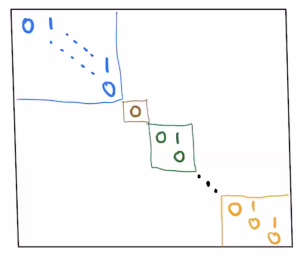
\includegraphics[width=0.25\textwidth]{Image 2 9232020.PNG}
    \end{center}
\end{itemize}
\end{proposition}
\begin{proof}
$1\implies 2$. Suppose that $Tv=\lambda v$ for some $\lambda\neq 0$ and $v\neq 0$. Then $T^2 v=\lambda^2 v\neq 0$. Continue in this way we get $T^m v\neq 0$ so $T^m\neq 0$ a contradiction since $T$ is nilpotent.
\\
$4\iff 5\implies 1$ Easy
\\
$2\implies 4$ We skip it for now
\\
$1\implies 4$ By induction on $m$ such that $T^m=0$. $TV$ is $T$ invariant subspace. $T^{m-1}(TV)=0$. By the induction hypothesis, $TV$ has a basis of chains:
\begin{center}
   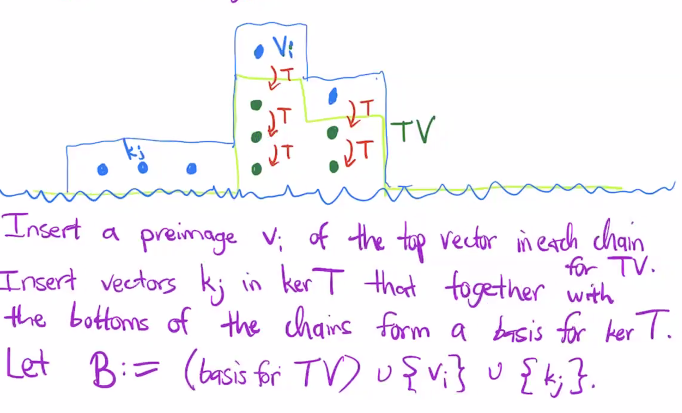
\includegraphics[width=0.25\textwidth]{Image 1 9232020.PNG}
\end{center}
Also, there are $\dim(\im T)+\dim(\ker T)=\dim V$ basis vectors in $B$. Thus $B$ is a basis since it has the right number of basis and is linearly independent.
\end{proof}
\begin{proposition}
$B$ is linearly independent. Suppose there were a linear dependence. If such a dependence existed, you can apply $T$ to get a dependence to the basis vectors in $TV$, so all the non-bottom coefficients are 0. Now the dependence is between the bottom vectors, which are a basis of $\ker T$, so their coefficients are zero too.
\end{proposition}
\begin{lemma}
If $T:V\ra V$ then $V=V_0\oplus W$. $T|_{V_0}$ is nilpotent and $T|_W$ is invertible. You can look at this as\\ $\begin{pmatrix}
\textrm{nilpotent}&\\
&\textrm{invertible}
\end{pmatrix}$
\end{lemma}
\begin{proof}
$V\subset TV\subset T^2V\subset...\subset T^nV$. The dimension can drop but it can only drop finitely many times so eventually the subspace has to stabilize. There exists $T^nV=T^{n+1}V=T^{n+2}V=...$. Define $V_0:=\ker(T^n)$ and $W:=T^n V$. Thus $W=TW$ so $T$ restricts to something on $W$ that's surjective so $T|_W$ is invertible. $T_{V_0}$ is nilpotent. $\ker(T^n)\cap W=\{w\in W:T^nw=0\}$ since $T|_W$ is injective. $\dim(\ker T^n)+\dim(\im T^n)=\dim V$. Thus $V_0\oplus W$ must be all of $V$.
\end{proof}
\begin{definition}[Jordan Block]
$\begin{pmatrix}\lambda\end{pmatrix},\;\begin{pmatrix}\lambda&1\\&\lambda\end{pmatrix},\;\begin{pmatrix}\lambda&1&\\&\lambda&1\\&&\lambda\end{pmatrix}$
\end{definition}
\begin{theorem}
Let $T:V\ra V$ represent a matrix with Jordan blocks along the diagona, unique except for rearranging the blocks. For example:
\begin{center}
   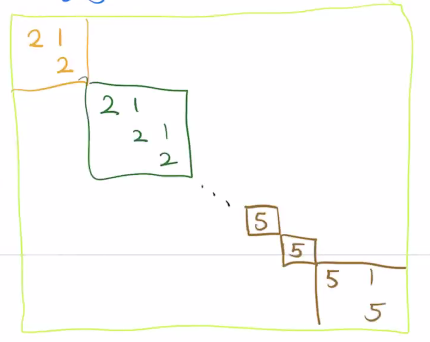
\includegraphics[width=0.25\textwidth]{Image 3 9232020.PNG}
\end{center}
\end{theorem}
The Jordan normal form is the closest you can get to diagonalizing a matrix. Any matrix $A\in \C^{n\times n}$ is similar to a matrix in Jordan normal form, unique except for rearranging the blocks.
\begin{proof}
Induction on $\dim V$. Suppose $\dim V\geq 1$. Let $\lambda\in \C$ be a zero of $p(t)$ so $\lambda$ is an eigenvalue. Replace $T$ by $T-\lambda I$ to assume $0$ is an eigenvalue. $V=V_0\oplus W$ where $V_0\neq 0$ so $\dim W<\dim V$ $T|_W$ has a JNF by the induction hypothesis. $T|_{V_0}$ has a JNF since it's nilpotent (proposition 59) \\
Uniqueness. Look at the number of $m\times m$ blocks with diagonal entry $\lambda$ is determined by $\dim\ker(T-\lambda I), \dim\ker((T-\lambda I)^2)$
\end{proof}
\begin{definition}
$v\in V$ is a generalized eigenvector with respect to eigenvalue $\lambda$ if $(T-\lambda I)^m V=0$ for some $m$. Let $V_\lambda =\{\textrm{generalized eigenvectors with eigenvalue}\lambda\}$
\end{definition}
\begin{corollary}
If $p(t)=(t-\lambda_1)^{e_1}...(t-\lambda_r)^{e_r}$ with $\lambda_i$ distinct. Then $V=V_{\lambda_1}\oplus V_{\lambda_2}\oplus...\oplus V_{\lambda_r}$ with dimensions $n=e_1+...+e_r$ where $e_i$ is the number of diagonal entries equal to $\lambda_i$ which is equivalently equal to the sum of sizes of blocks with diagonal $\lambda_i$. Also $\dim\ker(T-\lambda I)$ is the number of blocks with diagonal $\lambda$. $\ker(T-\lambda I)$ is the eigenspace of $\lambda$.
\end{corollary}
\section{September 24, 2020}
\begin{definition}
Let $x$ and $y$ be vectors. Then $x\cdot y=\begin{pmatrix}
x_1&...&x_n
\end{pmatrix}\begin{pmatrix}
y_1\\...\\y_n
\end{pmatrix}$. Observe that $|x\cdot y|=|x||y|\cos\theta$ where $\theta$ is the angle between $x$ and $y$.
\end{definition}
\begin{definition}
$|x|=\sqrt{x\cdot x}$
\end{definition}
\begin{definition}
$x\perp y$ means $x\cdot y=0$.
\end{definition}
\begin{definition}[An orthonormal basis]
Suppose we have $v_1,v_2,...,v_n\in \R^n$. This is an orthonormal basis if and only if $v_i\cdot v_j=\delta_{ij}$ where $\delta_{ij}$ is the Kronecker delta function. This is equivalent to $|v_i|=1$ and $v_i\perp v_j$ for all $i\neq j$.
\end{definition}
\begin{theorem}
The following are equivalent for $A\in \R^{n\times n}$:
\begin{itemize}
    \item $|Ax|=|x|$
    \item $(Ax)\cdot(Ay)=x\cdot y$
    \item $A^tA=I$
    \item The columns of $A$ form an orthonomral basis
\end{itemize}
\end{theorem}
\begin{proof}
$1\implies 2$ Use $x\cdot y=(|x+y|^2-|x|^2-|y|^2)/2$.\\
$2\implies 1$ Use $|x|=\sqrt{x\cdot x}$\\
$2\iff 3$ $x^tA^tAy=x^ty$ for all $x,y$ and in particular these is best seen by letting $x$ and $y$ be standard basis vectors.\\
$3\iff 4$ $(A^tA)_{ij}=\sum_k A^t_{ik}A_{kj}=\delta_{ij}$ $\iff$ $A^tA=I$
\end{proof}
\begin{definition}[Orthogonal Matrices]
If any of the conditions in theorem 70 hold for a matrix $A$, then $A$ is called an orthogonal matrix
\end{definition}
\begin{definition}
The orthogonal group $O_n$ is the set of orthogonal $n\times n$ matrices.
\end{definition}
\begin{proposition}
$O_n$ is a subgroup of $GL_n(\R)$
\end{proposition}
\begin{proof}
Use condition three of theorem 70
\end{proof}
\begin{proposition}
If $A$ is an orthogonal matrix then the determinant of $A$ is plus or minus one. For each $n\geq 1$, both values are possible.
\end{proposition}
\begin{proof}
$A^tA=I$. Take the determinant of both sides to get $\det(A)^2=1$. The determinant must be a second root of unity of 1 so $\det(A)=\pm 1$. The $I_n$ has determinant $1$ for all $n$ and the matrix that's $I$ everywhere except for the entry in the first row and column where it is negative 1.
\end{proof}
\begin{definition}
The special orthogonal group is the set of orthogonal matrices of determinant 1. It's the kernel of the determinant homomorphism restricted to $O_n$. $[O_n:SO_n]=2$.
\end{definition}
\begin{example}
Consider $n=2$. What are the possible orthonomal bases for $\R^2$?. The first vector has to be in the unit circle so it can be expressed as $\begin{pmatrix}
\cos\theta\\\sin\theta
\end{pmatrix}$. The second vector is either $\begin{pmatrix}
-\sin\theta\\\cos\theta
\end{pmatrix}$ or $\begin{pmatrix}
\sin\theta\\-\cos\theta
\end{pmatrix}$
\end{example}
\begin{corollary}
$O_2=\{\begin{pmatrix}
c&-s\\s&c
\end{pmatrix},\begin{pmatrix}
c&s\\s&-c
\end{pmatrix}\}$. All the matrices of the first type have determinant one and all the ones of the second type have determinant negative one. $SO_2=\{\begin{pmatrix}
c&-s\\s&c
\end{pmatrix}\}$. This is isomorphic to the units in $\C$.
\end{corollary}
\begin{proposition}
If $A\in S$ where $S$ is the nontrivial coset of $SO_2$ in $O_2$ which is $\{\begin{pmatrix}
c&s\\s&-c
\end{pmatrix}\}$ then $A$ is a reflection in some line $L$ through the origin (at angle $\theta/2$).
    \begin{center}
        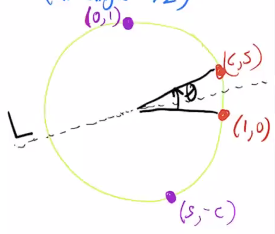
\includegraphics[width=0.25\textwidth]{Image 1 9252020.PNG}
    \end{center}
\end{proposition}
\begin{proof}
This matrix has eigenvalues 1 and -1. Take unit eigenvectors $v$ and $w$. We claim that $v\perp w$. $(Av)\cdot (Aw)=v\cdot w=v\cdot -w=-(v\cdot w)$. This is possible if and only if $v\cdot w=0$.
\end{proof}
What happens in three dimensions? Start with a unit vector $u\in \R^3$ and an angle $\theta$. Let $u^\perp$ be the set of all vectors in $\R^3$ that are perpendicular to $u$. This set forms a plane. Use the below image to deduce what a rotation is:
    \begin{center}
        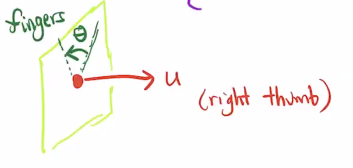
\includegraphics[width=0.25\textwidth]{Image 2 9252020.PNG}
    \end{center}
$\rho(u,\theta):=$ the linear operator $\rho:\R^3\ra\R^3$ such that $\rho(u)=u$ and $\rho_{u^\perp}$ is a counterclockwise rotation by $\theta$. It corresponds to a 3 by 3 matrix.
\begin{theorem}
The $3\times 3$ rotation matrices are $SO_3$
\end{theorem}
\begin{proof}
First we show that the set of $\rho$s is a subset of $SO_3$. Let $\rho$ be a rotation $\rho(u,\theta)$. Choose an orthonormal basis $(u,v,w)=P\in O_3$.
    \begin{center}
        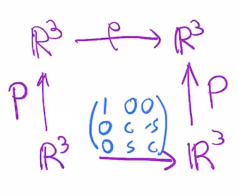
\includegraphics[width=0.25\textwidth]{Image 3 9252020.PNG}
    \end{center}
    $\rho=P\begin{pmatrix}
1&&\\&\cos\theta&-\sin\theta\\&\sin\theta&\cos\theta
\end{pmatrix}P^{-1}$ which is in $SO_3$. Since $SO_3$ is a normal subgroup of $O_3$ (it's the kernel of a homomorphism), $\rho\in SO_3$. Next time we will show the other inclusion.
\end{proof}
\section{September 28, 2020}
\begin{theorem}
$SO_3=\{3\times 3$ rotation matrices $\rho_{(u,\theta)}\}$.
\end{theorem}
\begin{proof}
We already showed that each 3$\times$3 rotation matrix $\rho_{(u,\theta)}$ is in $SO_3$. Suppose $A\in SO_3$. Then $A^tA=I$ and $\det A=1$. First, $1$ is an eigenvalue of $A$.  $\det(A-I)=\det(A-I)^t=\det(A^t-I)=\det(A^{-1}-I)=\det(A(A^{-1}-I))=\det(I-A)=-\det(A-I)$ so the determinant is zero. By performing an orthogonal change of basis, WLOG, $u=\begin{pmatrix}
1\\0\\0
\end{pmatrix}.$ Then $u^\perp=\begin{pmatrix}
0\\*\\*
\end{pmatrix}$ is $A$-invariant so $A=\begin{pmatrix}
1&&\\&*&*\\&*&*
\end{pmatrix}$. The two by two asterisk portion must also be orthogonal for $A$ to be orthogonal. Hence this little matrix is in $S0_2$. So $A$ is a rotation of $\R^3$.
\end{proof}
\begin{definition}
Let $f:\R^n\ra\R^n$. This map is called an isometry if it preserves distances. $|f(x)-f(y)|=|x-y|$ for all $x,y\in \R^n$.
\end{definition}
\begin{example}
\begin{itemize}
    \item An orthogonal linear operator. $\R^n\ra[A]\R^n$, $x\mapsto Ax$ preserves distance for $A\in O_n$.
    \item "translation by $b$" $\R^n\ra[t_b]\R^n$ for $b\in \R^n$, $x\mapsto x+b$.
\end{itemize}
\end{example}
\begin{theorem}
Every isomstry $f:\R^n\ra\R^n$ is $t_bA$ for some unique $b\in \R^n$ and $A\in O_n$.
\end{theorem}
\begin{lemma}
An isometry that fixes 0 is a linear operator.
\end{lemma}
\begin{proof}
First, $f$ preserves distances and zero. We can express dot products in terms of 0 and distances. $u\cdot v=\frac{1}{2}(|u|^2+|v|^2-|u-v|^2)$. If an operator preserves distances, then it preserves dot product, $f(u)\cdot f(v)=u\cdot v$ so $f$ preserves dot product. We can express sums in terms of dot products. $z=x+y\iff (z-x-y)\cdot(z-x-y)\iff z\cdot z-2x\cdot z-...=0$ so $f$ preserves taking sums. Similarly $f$ preserves scalar multiplication by each $c\in \R$.
\end{proof}
\begin{proof}[Proof of theorem]
Let $b=f(0)$. Then $t_b^{-1}f$ is an isometry mapping 0 to 0. so $t^{-1}_bf=A$ for some orthogonal matrix $f=t_bA$. If $f=t_bA$ then $f(0)=t_bA(0)=t_b=b$ so $b$ is determined by $f$, and then $A=t^{-1}_bf$ is uniquely determined too.
\end{proof}
\begin{definition}
The set of all isometries from $\R^n$ to itself is denoted $M_n$. $M_n=\{t_bA:A$ orthogonal $t_b$ translation $\}$. which maps $x\mapsto Ax+b|A\in O_n, b\in \R^n$. This is a subgroup of the group of permutations of the plane. The set of translations over $\R^n$ (which is isomorphic to the additive group of $\R^n$) is a normal subgroup of $M_n$ and the group of orthogonal operators is a subgroup of $M_n$. The mapping $\R^n\times O_n\ra M_n$ under $(t_b,A)\mapsto t_bA$ is a bijection between the two sets but it is not an isomorphism since $t_b$ and $A$ don't commute in general. Instead, $At_b=t_{A(b)}A$.
\end{definition}
Let $M_n:\ra[\pi]O_n$ where $(x\mapsto Ax+b)\mapsto A$. This is a homomorphism. The kernel is going to be the translations which proves that the translations are a normal subgroup.
\begin{definition}
If $x\mapsto Ax+b$ is \vocab{orientation preserving} it has $\det A=1$ and \vocab{orientation reversing} if $\det A=-1$.
\end{definition}
\begin{theorem}
Every isometry of $\R^2$ is one of the following:
\begin{itemize}
    \item translation $x\mapsto x+b$
    \item rotation around some point
    \item reflection across $r_l$ a line $l$. The line is not necessarily through zero.
    \item glide reflection: $t_br_l$ for $b$ parallel to $l$.
\end{itemize}
\end{theorem}
\begin{proof}
Let $f$ be an isometry under which $x\mapsto Ax+b$. If $f$ is orientation preserving: If $A=I$, then $f$ is a translation. If $A\neq I$ then $f$ has a fixed point. We need to solve $Ax+b=x$ where $A=\begin{pmatrix}
\cos\theta&-\sin\theta\\\sin\theta&\cos\theta
\end{pmatrix}$. We need to solve $(A-I)x=-b$. If $A$ is a rotation, then it does not fix any nonzero vector so $\ker(A-I)=\{0\}$ so $A-I$ is invertible so we can find a fixed point for $A$.
\end{proof}
\section{September 30, 2020}
Last time, we stated that every isometry $f$ or $\R^2$ is one of the following: $x\mapsto x+b$, rotation, reflection $t_b,r_l$, glide reflection $t_br_l$ for some line $l$ and nonzero vector $b$ parallel to $l$.
\begin{proof}
$f=t_bA$ where $A$ is a reflection in a line $L$ which contains 0. Change the origin to $b/2$. This is equivalent to $t^{-1}_{b/2}ft_{b/2}=t_{-b/2}t_bAt_{b/2}=t_{b/2}t_{A(b/2)}A=t_mA$ where $m=\frac{1}{2}(b+Ab)$. If $m=0$, this is a reflection and if $m\neq 0$, then this is a glide reflection.
\end{proof}
\begin{definition}
A subgroup $G$ or $\R$ is discrete if and only if there exists $\eps>0$ such that every nonzero element $g\in G$ satisfies $|g|\geq \eps$. Then if $g,h\in G$ are distinct, then $|g-h|\geq\eps$.
\end{definition}
\begin{theorem}
Every discrete subgroup $G\leq \R$ is $\{0\}$ or $a\Z$ for some $a\in\R_{>0}$.
\end{theorem}
\begin{proof}[Idea of proof]
Assume $G\neq\{0\}$. Then there exists $b\neq0$ and thus $-b$ or $b$ is positive. There is a least positive real number $a$ since between since the distance between any two points is greater than $\eps$. If there is $b\in G$ and $b\notin a\Z$, then $b'=b-\lfloor \frac{b}{a}\rfloor a$ satisfies $0<b'<a$, a contradiction.
\end{proof}
\begin{definition}[Finite subgroups of $O_2$]
Let $x$ be the rotation by $2\pi/n$ about $O$ and $y$ the reflection in a line $l$ which contains 0. $C_n=<x>$ and $D_n$ is the subgroup of $O_2$ generated by $x$ and $y$.  This is equal to $<x,y:x^n=1,y^2=1,yx=x^{-1}y>=\{1,x,x^2,...,x^{n-1},y,xy,...,x^{n-1}y\}$ and these elements are distinct.
\end{definition}
\begin{fact}
$D_1\cong C_2,\; D_2\cong C_2\times C_2,\; D_3\cong S_3$ for $n\geq 3$, $D_n$ is the set of symmetries of a regular $n$-gon.
\end{fact}
\begin{fact}
Group game: you name all the groups of order 1, I name all the groups of order 2, you name all the groups of order 3,...
\end{fact}
\begin{theorem}
Every finite subgroup $H\leq SO_2$ is $C_n$ for some $n\geq 1$.
\end{theorem}
\begin{proof}
Let $S=\{\theta\in\R;\rho_\theta\in H\}\leq \R$. Then $S$ is discrete (it has finitely many elements in any bounded interval) so $S=a\Z$ for some $a\in \R_{>0}$. Also $2\pi\in S$ so $2\pi=na$ for some $n\in \Z_{n>0}$ so $a=2\pi/n$ so $S=(\frac{2\pi}{n})\Z$ which is equal to the set of rotations by multiples of $2\pi/n$ which is $C_n$
\end{proof}
\begin{theorem}
Now, we're going to classify all subgroups $\leq O_2$. Every subgroup $G\leq O_2$ is $C_n$ or $D_n$ for some $n\geq 1$.
\end{theorem}
\begin{proof}
We split this into two cases:
\begin{itemize}
    \item[Case 1:] $G\subset SO_2$. Then $G=C_n$ for some $n$, by the theorem 94.
    \item[Case 2:] $G$ is not a subset of $SO_2$. There are two elements of $O_2/SO_2$ (remember that $SO_2=\ker\det:\R^{2\times 2}\ra \{-1,1\}$). Let $H=\ker(G\ra\{\pm 1\})$. Then $G\ra\{\pm\}$ has two nonempty fibers. Namely, $H$ and $Hr$ for some reflection $r$. Here, $H\subseteq SO_2$ so $H=C_n$ for some $n$. Then $G$ is generated by $C_n$ and a reflection $r$ so $G\cong D_n$.
\end{itemize}
\end{proof}
Discrete subgroups of $O_2$ are the same as finite subgroups of $O_2$. What are the finite subgroups of $M_2$, the full isometry group? (remember that this is generated by the translations and $O_2$.
\begin{theorem}
Every finite subgroup of $M_2$ has a fixed point $x$ (Taking $x$ to the origin shows that $G\cong C_n$ or $D_n$ for some $n\geq 1$).
\end{theorem}
\section{October 2, 2020}
Today, we will classify the discrete subgroups of $M_2$. Last time we determined the finite subgroups of $O_2$: the cyclic groups and the dihedral groups. It turns out that the discrete subgroups of $O_2$ are finite so they are $C_n$ and $D_n$ as well.\\
Let $S$ be a subset of $\R^n$. Call $s\in S$ \vocab{isolated} if some open ball around $s$ contains no other points of $S$. Call $S$ \vocab{discrete} if every point of $S$ is isolated. The discrete subgroups of $\R$ are $\{0\}$ and $a\Z$ for any $a\in\R_{>0}$. Today we will show the following:
\begin{theorem}
The discrete subgroups of $\R^n$ are $\{0\}$, $a\Z$, and $a\Z+b\Z$ for linearly independent $a,b\in \R^2$. The discrete subgroups of the third type are called full lattices.
\end{theorem}
\begin{proof}
Let $G\leq \R^2$ be a subgroup that is not the trivial group. Choose a one dimensional subspace $L$ such that $G\cap L\neq \{0\}$. Then $G\cap L=a\Z$ for some $a\in L-\{0\}$. If $G=a\Z$, then we're done. Otherwise, there's some other element $b$ in $G$ that's outside $G-a\Z$ closest to $L$. Observe that any bounded subset $B$ of $\R^2$ contains only finitely many elements of $G$. Using this fact and closure of subgroups, such a $b$ that's closest to $L$ exists. Then $G=a\Z+b\Z$ since otherwise, by shifting, the parallelogram with sides $a$ and $b$ would contain an element of $G$ closer to $L$ than $b$ is.
\end{proof}
\begin{theorem}
Every finite subgroup $G\leq M_2$ is isomorphic to to $C_n$ or $D_n$ for some $n\geq 1$.
\end{theorem}
\begin{proof}
We first prove that there is a finite set $S$ such that $gS=S$ for every $g\in S$. Form $G_s$ the $G$-orbit of $s$. Then $g(Gs)=(gG)s=Gs$\\
We now show there there is a unique point $x$ minimizing $|x-s_1|^2+|x-s_2|^2+...+|x-s_n|^2$. This is equal to $(x-s_1)\cdot (c-s_1)+...+(x-s_n)\cdot (x-s_n)=n(x-\frac{s_1+s_2+...+s_n}{n})^2+$ constant that depends on the $s_i$ but not on $x$. The first term is minimized when $x=\frac{s_1+...+s_n}{n}$, which is the centroid of the set $S$.\\
$x$ is a fixed point $(gx=x)$ for all $g\in G$. $g$ preserves $S$ and preserves distances so $g$ must preserve $x$.\\
Now, we show $G$ is isomorphic to $C_n$ or $D_n$. Make $x$ the new origin. Then $G\leq O_2$. The resule follows from the fact that all finite subgroups of $O_2$ are $C_n$ and $D_n$.
\end{proof}
\begin{definition}
Let $G\leq M_n$. Identify $M_n$ with $\{(A,b):A\in O_n, b\in\R^n\}\subseteq\R^{n^2+n}$. We can view $G$ as being a subset of this big Euclidean space. Call $G$ discrete if and only if it is discrete as a subset of $\R^{n^2+n}$. This is equivalent to there not existing a sequence $g_1,g_2,...$ of distinct elements of $G$ converging to 1.
\end{definition}
\begin{proposition}
Each $A\in\bar{G}$ maps $L$ to $L$. $L$ is the set of translations in $\bar{G}$.
\end{proposition}
\begin{proof}
Suppose $A\in\bar{G}$ and $t_a\in L$. We need to show that $t_{A_a}\in L$. By definition, $A$ is the image of some $t_bA\in G$. Then $(t_bA)t_a(t_bA)^{-1}\in G$. $t_bAt_aA^{-1}t^{-1}_b=t_bt_{Aa}A^{-1}t_{-b}=t_bt_{Aa}t_{-b}=t_{Aa}$ since translations commute.
\end{proof}
\section{October 5, 2020}
Let's make some things clear. Let $G$ be a discrete subgroup of $M_2$. $\bar{G}=\pi(G)$, the point group of $G$ and $L=\ker\pi$
\begin{example}
If you take a rhombic lattice, every element of $\bar{G}$ preserves this lattice. Thus $\bar{G}\leq D_2$
\end{example}
\begin{theorem}
Let $G\leq M_2$ be discrete.
\begin{enumerate}
    \item[(1)] $L$ is a discrete subgroup of $\R^2$
    \item[(2)] If $L\neq \{0\}$, then $\bar{G}=C_n$ or $D_n$ where $n$ is 1,2,3,4 or 6.
    \item[(3)] If $L=\{0\}$ then $G$ is finite.
\end{enumerate}
\end{theorem}
\begin{proof}
(1): A subset of a discrete set is discrete. \\
(2): Let $a$ be the shortest nonzero vector in $L$. If $\rho_\theta$ is a rotation in $\bar{G}$, then $\rho a\in L$. Then $\theta\geq 2\pi/6$ since otherwise $\rho a-a$ is shorter than $a$, a contradiction. Thus $\bar{G}$ is a discrete subgroup of $O_2$. So $\bar{G}=C_n$ or $D_n$ and $n\leq 6$. If $n=5$, then $a+\rho_{2(2\pi/5)}a$ is shorter than $a$, contradiction. If you have a square lattice, $n=4$ is legit. \\
(3) Suppose $L=\{0\}$. Let $H$ be the subgroup of orientation preserving isometries in $G$. If $H$ has rotations around two different points, then there exists a translation in $H$. But that's impossible since $L$ contains no translations. Thus, after changing origin, $H$ is a discrete subgroup of $SO_2$, so $h\cong C_n$. Then $G$ is finite: $|G|\leq 2|H|$. So $G\cong C_n$ or $D_n$.
\end{proof}
\subsection{Group Action}
Each $A\in GL_n$ gives a bijection $\R^n\ra[A]\R^n$. Package them all into one function. $GL_n\times \R^n\ra\R^n$, $(A,\vec{x})\mapsto A\vec{x}$. We say $GL_n$ acts on $\R^n$. Similarly, we can say that $S_n$ acts on $\{1,2,...,n\}$. $M_2$ acts on $\R^2$.
\begin{definition}
Let $G$ be a group and $S$ a set. An action of $G$ on $S$ is a function $G\times S\ra S$, $(g,s)\mapsto gs$. It satisfies the following two properties:
\begin{enumerate}
    \item[(1)] $1s=s$ for all $s\in S$.
    \item[(2)] $(gh)s=g(hs)$ for all $g,h\in G$ and $s\in S$.
\end{enumerate}
\end{definition}
Let $G$ act on $S$. Fix $g\in G$, get a permutation of $S$. $m_g:S\ra S$, $s\mapsto gs$. The inverse is $m_{g^{-1}}$. This is easy to show using the two axioms of group actions above.\\
The map $G\ra Perm(S)$, $g\mapsto m_g$ is a group homomorphism: $m_gm_h=m_{gh}$ because $m_g(m_h(s))=g(hs)=(gh)s=m_{gh}s$ for all $s\in S$. \\
Giving an operation of $G$ and $S$ is the same as giving a a homomorphism from $G$ to the permutation group of $S$.
\begin{definition}
The operation  is faithful if the only $g\in G$ that acts triviall on $S$ is the identity of $G$. I.e. $gs=s$ for all $s$ implies that $g=1$. This is equivalent to $\ker(G\ra Perm(S))=\{0\}$, or that this map is injective
\end{definition}
\begin{definition}
Suppose $G$ acts on $S$, $s\in S$. The orbit of $s$ is $O_s=Gs=\{gs:g\in G\}$. This is a subset of $S$.
\end{definition}
\begin{definition}
The stabilizer of $s$ is the set $\Stab_G(s)=\{g\in G: gs=s\}$. This is not the kernel of $G\ra Perm(S)$ since this is the set that stabilizes all $s\in S$. The kernel of this homomorphism is $\cap_{s\in S}\Stab_G(s)$.
\end{definition}
\begin{example}
Take $S_n$. The stabilizer of any element is isomorphic to $S_{n-1}$.
\end{example}
\begin{proposition}
The orbits form a partition of $S$. This can be proved by showing that the the orbit defines an equivalence class on $S$.
\end{proposition}
\begin{proposition}
Let $G$ act on $S$ and $s\in S$. Let $H=\Stab(S)$. There exists a bijection between $G/H\ra[\eps]O_s$, $gH\mapsto gs$.
\end{proposition}
\begin{proof}
For $g,\gamma\in G$, $\gamma s=gs$ if and only if $g^{-1}s=s$, or equivalently that $g\equiv \gamma (\Stab(s)$. Thus the mapping above is well-defined and the mapping is injective. The map is trivially surjective.
\end{proof}
\begin{corollary}
$|O_s|=(G:\Stab(s))$ or equivalently $|O_s||\Stab(s)|=|G|$. This is called the orbit stabilizer formula. For any $H\leq G$, normal or not, $G$ acts on $G/H$ by $g$ maps $C\in G/H$ to $gC$. This turns out to be transitive, stabilizer of the coset $H\in G/H$ is $H$.
\end{corollary}
\section{October 7, 2020}
The orbit of $s_1$ is in bijection with $G/H_1$ where $H_1=\Stab(s_1)$. Suppose $s'=as$. Then $\Stab(s')=a\Stab(s)a^{-1}$. Recall that $S0_3$ are the rotations in $\R^3$ that fix the origin.
\begin{theorem}
The finite subgroups of $SO_3$ are the following:
    \begin{center}
        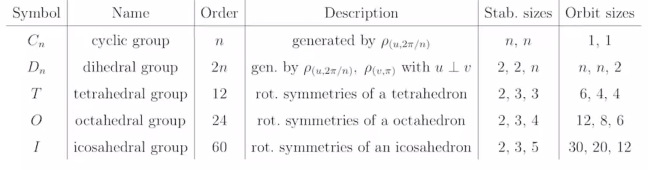
\includegraphics[width=0.35\textwidth]{Image 1 1072020.PNG}
    \end{center}
\end{theorem}
Let $G$ be a finite subgroup. For $g\in G$, $g$ fixes two unit vectors (along the axis of rotation). Let $$P=\bigcup_{g\neq 1}\{\textrm{poles of g}$$. If $G=C_n$ there are two poles. If $G=D_n$, there are 2+2n poles.
\begin{lemma}
If $p$ is a pole and $g\in G$, then $gp$ is a  pole.
\end{lemma}
\begin{proof}[Proof of Theorem 110]
Since $p$ is a pole, $\Stab(p)\neq \{1\}$. Then $\Stab(gp)=g\Stab(p)g^{-1}\neq\{1\}$. Thus $G$ acts on $\mathbb{P}$, the set of poles of $G$. Let $N=|G|$. Let $r_i=|\Stab(p_i)|$ and $n_i=O_{p_i}$. Then $n_ir_i=N$. We know that $1<r_i\leq N$. We are going to count pairs $(g,p)$ where $g\neq 1$ and $p$ is a pole of $g$. This is the same as $$\sum_{g\in G\cap g\neq 1}2=2N-2=\sum_{p\in\mathbb{P}}|(\Stab(p)|-1)=N\sum_i(1-r_i)$$ Thus, $\sum_i(1-r_i)=2-2/N\in[1,2)$. In the case of two orbits, $\frac{1}{r_1}+\frac{1}{r_2}=\frac{2}{N}\geq \frac{1}{N}+\frac{1}{N}$ so $r_i=N$. Thus $n_1$ and $n_2$ are equal to 1 by the orbit stabilizer formula. Geometrically, the total number of poles is 2 and each pole is fixed by the whole group. If there are three orbits, $N-(\frac{1}{r_1}+\frac{1}{r_2}+\frac{1}{r_3})=2-\frac{2}{N}$. Thus $\frac{1}{r_1}+\frac{1}{r_2}+\frac{1}{r_3}=1+\frac{2}{N}$. If $r_1\geq 3$, then the left hand side is less than or equal to $\frac{1}{3}+\frac{1}{3}\frac{1}{3}=1$. If $r_2\geq 4$ then the left hand side is less than or equal to $\frac{1}{2}$ a contradiction. Subcase $r_2=2:$ Then $\frac{1}{r_3}=\frac{2}{N}$ so $r_3=\frac{N}{2}$ so that $G=D_{\frac{N}{2}}$. Subcase $r_2=3:$ $\frac{1}{r_3}=\frac{1}{6}+\frac{2}{N}$. Subsubcase: $r_3=4$. $\frac{1}{4}=\frac{1}{6}+\frac{2}{N}$ so $N=24$. The $r_i$ are $2,3,4$ (stabilizer sizes), The $n_i$ are 12,8,6j (orbit sizes). Thus $G$ preserves the set of vertices of an octahedron.
\end{proof}
\section{October 9. 2020}
What are the finite subgroups of $O_3$? $O_3$ is generated by $SO_3$ and $\{\pm I\}$ with intersection $\{I\}$ since $\det(-I)=(-1)^3=-1$ and $gh=hg$ for all $g\in SO_3$ and $h\in\{\pm I\}$, so $O_3\cong SO_3\times \{\pm I\}$. We can classify the finite subgroups of $O_3$ using Goursat's lemma.
\begin{lemma}[Goursat's lemma]
Let $G$ and $G'$ be groups and let $H$ be a subgroup of $G\times G'$ such that the two projections $p_1:H\ra G$ and $p_2:H\ra G'$ are surjective ($H$ is a subdirect product of $G$ and $G'$). Let $N$ be the kernel of $p_2$ and $N'$ the kernel of $p_1$. Once can identify $N$ as a normal subgroup of $G$ and $N'$ as a normal subgroup of $G'$. Then the image of $G$ in $G/N\times G'/N'$ is the image of an isomorphism $G/N\cong G'/N'$
\end{lemma}
Two actions of $G$ on $\mathbb{G}$: left multiplication: $g$ does $m_g:\mathbb{G}\ra G$, $x\mapsto gx$. We get a homomorphism $G\ra Perm(\mathbb{G})$, $g\mapsto m_g$. What is the kernel? If $g$ is the kernel, then $m_g=\id$, so $m_g(1)=1$, so $g=1$. Thus $\ker=\{1\}$. Cayley's theorem says that if $|G|=n$, then $G$ is isomorphic to a subgroup of $S_n$. Conjugation: $g$ does $x\mapsto gxg^{-1}$. The orbit of $x$ is $\{gxg^{-1}:g\in G\}$ which is the \vocab{conjugacy class} of $x$. The stabilizer of $x$ is $\{g\in G:gxg^{-1}=x\}=\{g\in G:gx=xg\}=Z(x)$, the \vocab{centralizer} of $x$ (this is a subgroup). Then $|G|=|C(x)||Z(x)|$. $C(x)=\{x\}$ if and only if $Z(x)=G$ if and only if $x\in Z$, the center of $G$. The class equation is $|\mathbb{G}|=|C_1|+...+|C_k|=|Z|+|G|\sum_{x\notin Z}\frac{1}{|Z(x)|}$.
\begin{definition}
$G$ is a $p$-group if and only if $|G|$ is a power of $p$.
\end{definition}
\begin{definition}
An \vocab{Elementary Abelian p-group} is an Abelian group $G$ in which every element has order dividing $p$.
\end{definition}
\begin{example}
$C_p\times C_p\times C_p\cong \mathbb{F}_p^3$
\end{example}
\begin{proposition}
If $G$ is a nontrivial $p$-group, its center is not trivial
\end{proposition}
\begin{proof}
Given $|G|=p^e$ for some $e\geq 1$, each $|C_i|$ divides $p^e$ so it is a power of $p$. By the class equation, $p^e=|Z|+\sum(\textrm{ higher powers of p})$ so $p$ divides $|Z|$ (all those $C_i$ with $|C_i|=1$ go into the center).
\end{proof}
\begin{proposition}
If $|G|=p^2$, then $G$ is abelian
\end{proposition}
\begin{proof}
The trivial group is a proper subgroup of $Z$ which is a subgroup of $G$. If $|Z|=p$, choose $x\in G-Z$. Then $Z$ is a proper subgroup of $Z(x)$ since $x\in Z(x)$ so $|Z(x)|=p^2$, a contradiction since $x\in Z$ and $x\notin Z$.
\end{proof}
\begin{proposition}
If $|G|=p^2$, then $G\cong C_{p^2}$ or $G\cong C_p\times C_p$.
If every element of $G$ has order $p^2$, then $G$ is $C_{p^2}$. If there is an element of order $p$, then $G$ must $C_p\times C_p$
\end{proposition}
If $d$ is a divisor of $n$, then $n$ factors into $d$ and $\frac{n}{d}$. If $N$ is a normal subgroup of $G$, then $G$ decomposes into $N$ and $G/N$.
\begin{definition}
$n$ is a prime number if and only if $n>1$ and its only positive divisors are 1 and $n$.
\end{definition}
\begin{definition}
$G$ is a simple group if and only if $G\neq\{1\}$ and its only normal subgroups are itself and the trivial group.
\end{definition}
Next time, we'll prove that $I\cong A_5$ where $I$ is the icosahedral group and its also simple.
\section{October 13, 2020}
\begin{theorem}
$I\cong A_5$ and it is simple.
\end{theorem}
$I$ is the group of rotational symmetries of an icosahedron and it is a subgroup of $SO_3$.

\begin{tabular}{c|c|c|c|c}
    Pole directionn &  |Orbit| & Stabilizer & Elements in stabilizer & How man elts?\\
    midpoint of face & 30 & $C_2$ &$\rho_{(u,\pi)}$ & 15\\
    Center of face & 20 & $C_3$ & $\rho_{(u,2\pi/3)}$ & 20\\
    vertex & 12 & $C_5$ $\rho_{(u,2\pi/5)}$, $\rho_{(u,4\pi/6)}$ & 12, 12
\end{tabular}

The class equation gives $60=1+12+12+15+20$. If $N$ is a normal subgroup of $I$ then $N$ is the union of some of the conjugacy classes. But $|N|$ divides 60 so $N=\{1\}$ or $N=I$. This shows $I$ is simple. Now we show $I$ is isomorphic to $A_5$. Find a set of cardinality 5 that $I$ acts on. $I$ acts on a dodecahedron. $S:=$ the set of 5 cubes with vertices at the dodecahedron's vertices. $I$ acts on $S$. You get $\phi:I\ra Perm(S)$. But $\ker\phi$ is either 1 or $I$ since $I$ is simple. But $\ker\phi\neq I$ since $I$ doesn't act nontrivially on $S$. Thus $\phi$ is injective. Consider $I\ra S_5\ra[sgn]\{\pm\}$. Call this composition $\psi$. But $\ker\psi=\{1\}$ or $\ker\psi=I$. In the first case, $\psi:I\ra\{\pm\}$ is injective. But this is impossible since $|I|=60$ and $|\{\pm\}|=2$. Thus $\ker\psi=I$ so the image of all elements in $I$ is an even permutation, or $\phi(x)\in A_5$. Thus $I$ is isomorphic to $A_5$.

Next, we'll talk about conjugating in $S_n$.

Consider $p=(14)(253)\in S_5=Perm(\{1,2,...,5\}\cong Perm(\{a,b,...,3\})$ and $p'=(ab)(cde)\in Perm(\{a,b,...,3\})$. Define a bijection $\{1,2,...,5\}\ra\{a,b,...,e\}$. Then $qpq^{-1}=p'$. Instead of going between going between two different sets, consider the case where $q$ is the bijection from $\{1,...,5\}$ to itself so that $qpq^{-1}$ is conjugation. View $q$ as a "relabeling" of the numbers. Two elements are conjugate to each other if and only if the lengths of their cycles are the same. \\
The number of conjugacy classes in $|S_n|$ is the partition function of $n$. How many elements of $S_10$ are conjugate to $(123)(456)(789 {10})$. $|Z(x)|=2!\times 3\times 3\times 4$ the 2! comes from the number of ways to decide which 3 cycle comes first and the $3\times 3\times 4$ comes from how many ways there are to rotate the other cycles.
\section{October 14, 2020}
$S_4$ acts by conjugation on the conjugacy class of $(12)(34)$. Let $a=(12)(34), b=(13)(24), c=(14)(23)$. Get permutation representation $\phi: S_4\ra Perm(\{a,b,c\})\cong S_3$, $(12)\mapsto (bc), (123)\mapsto (acb), (12)(34)\mapsto 1$.  Thus $\phi$ is surjective. $|\ker\phi|=\frac{|S_4|}{|\im\phi|}=4$. In fact, $V=\ker\phi=\{1,a,b,c\}$. This is a normal subgroup. $|V|=p^2$ so it is either $C_4$ or $C_2\times C_2$. I know that the Klein group is $C_2\times C_2$.
\begin{example}
Is $A_4$ simple? No, because $V$ is a normal subgroup of $A_4$.
\end{example}
The conjugacy classes in $A_4$ are 1. the identity, 2. the 3 cycles, and 3. the product of disjoint 2 cycles. Is $(123)$ conjugate to $(213)$ in $S_4$? Yes, conjugation by (12). However, not in $A_4$. It's conjugate in $A_5$ though. If $n\geq 5$ then $\{\textrm{3 cycles in }A_n\}$ is one conjugacy class in $A_n$.
\begin{theorem}
If $n\geq 5$ then $A_n$ is simple. We did this last time for $n=5$ by showing it's isomorphic to the icosahedral group.
\end{theorem}
\begin{proof}
Suppose $N$ is not the trivial group and is normal in $A_n$. We need to show $N=A_n$. Choose $x\in N$, $x\neq 1$. We need only show that $A_n$ contains a 3-cycle. In that case, all 3-cycles are in $N$. Since the 3-cycles generate $A_n$ from a problem in PSET 1, it will follow that $N=A_n$.
\begin{enumerate}
    \item[Case 1:] $x$ has order $l\geq 5$ where $l$ is prime. Let $x=(1,2,3,4,5,...,l)y$ where $y$ stabilizes 1,2,3,4,5. Let $g=(432).$ then $gxg^{-1}x^{-1}=(245)$. The commutator is a 3-cycle.
    \item[Case 2:] $x$ has order 3. If $x$ contains is a 3-cycle then we're done. If not, then let $x=(123)(456)y$. Let $g=(432)$. Then $gxgg^{-1}x^{-1}=(15243)$. The commutator has order 5. Go back to case 1.
    \item[Case 3a:] $x$ has order 2 and it contains a 1-cycle. Since it is an even permutation, $x$ must contain at least two 2-cycles, say $x=(12)(34)(5)y$. Let $g=(531)$. Then $gxg^{-1}x^{-1}=(15243)$. The commutator has order 5 so go back to case 1.
    \item[Case 3b:] $x$ has order $l=2$ and contains no 1-cycles. Since $n\geq 5$, $x$ contains no more than two 2-cycles. Say $x=(12)(34)(56)y$. Let $g=(531).$ Then $gxg^{-1}x^{-1}=(153)(246)$. The commutator has order 3 and we go back to case 2. These are the possiblities for an even permutation of prime order, so the proof is complete.
\end{enumerate}
\end{proof}
\begin{definition}[The Normalizer]
Suppose $G$ acts on itself by conjugation. Then $G$ acts on the set of subsets of $G$. For $H\leq G$, $\Stab(H)=\{g\in G:gHg^{-1}=H\}$. This is also called the normalizer of $H$, $N(H)$.
\end{definition}
\begin{example}
Let $G=S_3$. What is the normalizer of $H=<(12)>$? $|G|$ is the product of the conjugates of $H$ and the order of the normalizer of $H$. Thus $|N(H)|=2$ so $N(H)=\{1,(12)\}$ so $N(H)=H$
\end{example}
\begin{theorem}[Lagrange's Theorem]
If $H\leq G$ then $|H|$ is a divisor of $|G|$. If $d$ divides $|G|$ must $G$ have a subgroup of order $d$? No! Then This would lead to too many elements.
\end{theorem}
However, if $d$ is a prime power, then the answer to the above question is yes.
\begin{theorem}[1st Sylow Theorem]
Suppose $|G|=n=p^em$ where $p$ doesn't divide $m$. Then there is a subgroup $H$ of $G$ with $|H|=p^e$.
\end{theorem}
\section{October 16, 2020}
\begin{theorem}[Cauchy's Theorem in Group Theory]
If $p$ divides $|G|$ then $G$ has an element of order $p$.
\end{theorem}
\begin{proof}[Cauchy's theorem for a finite Abelian Group]
Let $|G|=n$ and $x_1,...,x_n$ elements of $G$. We get a surjective homomorphism $<x_1>\times <x_2>\times...\times<x_n>\ra G$ where $y_1,y_1,...,y_n\mapsto y_1+...+y_n$. If $p$ divides $|G|$ then $p$ divides $|<x_1>\times...\times <x_n>|$ so $p$ divides $|<x_i>|$ for some $i$. So $<x_i>$ contains a copy of $C_p$.
\end{proof}
\begin{proof}[Proof of Sylow Theorem 1]
By induction on the order of $G$.
Assume that $p$ divides $|G|$. Use the class equation: $$|G|=|Z|+\sum_{\textrm{conjugacy classes}} |C(x)|$$.
\begin{enumerate}
    \item[Case 1:] Some $|C(x)|>1$ is not divisible by $p$. Then $|G|=|C(x)||Z(x)|$ (orbit stabilizer theorem). This shows that $Z(x)$ is divisible by the same power of $p$ as $|G|$, so a Sylow $p$-subgroup of $Z(x)$ is a Sylow $p$-subgroup of $G$. By the induction hypothesis, $Z(x)$ has a Sylow $p$-subgroup.
    \item[Case 2:] Every $|C(x)|>1$ is divisible by $p$. Class equation says that $|Z|$ is divisible by $p$. Cauchy's theorem for $|Z|$ says that there exists $C_p\leq Z$. Get $G\ra[\pi]G/C_p$. Let $S$ be the Sylow $p$-subgroup of $G/C_p$ (which exists from the inductive hypothesis) so $|S|=p^{e-1}$ since $|G|=p^em$ and $|G|/|C_p|=p^{e-1}m$. Then $|\pi^{-1}(S)|=|\ker\pi||S|=p^e$ so this is a Sylow $p$ subgroup for $G$.
\end{enumerate}
\end{proof}
\begin{proof}[Proof of Cauchy's theorem for any finite group]
We are given that $p$ divides $|G|$. We want to know that $G$ contains a subgroup of order $p$. It has a Sylow $p$-subgroup. If $x\in S$ then the order of $x$ is $p^k$ for some $k$. Then $x^{p^{k-1}}$ has order $p$.
\end{proof}
\begin{theorem}[2nd Sylow Theorem]
Fix a finite group $G$ and a prime $p$
\begin{enumerate}
    \item The Sylow $p$ subgroups are conjugates of each other.
    \item Every $p$ subgroup of $G$ is contained in a Sylow $p$-subgroup.
    \item The Sylow $p$ subgroups are normal if and only if $G$ has only one Sylow $p$ subgroup
\end{enumerate}
\end{theorem}
\begin{lemma}
Let $X$ be a finite set and $P$ a $p$-group acting on $X$. Then $X^P=\{x\in X:px=x\forall p\in P\}$. Then $|X|\equiv|X^P|\mod{p}$.
\end{lemma}
\begin{proof}
Every orbit in $X-X^P$ has size $p^a$ for some $a\geq 1$. Add their sizes to get $|X-X^P|$ is divisible by $p$.
\end{proof}
\begin{proof}[Proof of 2nd Sylow Theorem]
\begin{enumerate}
    \item[2.] Let $S$ be a Sylow $p$-subgroup. Let $P$ be any $p$-subgroup. Let $X=G/S$ so $|X|=|X^P|=m\neq 0(\mod{p})$ so there exists $x\in X$ fixed by $P$. Then $P\leq \Stab(x)=aSa^{-1}$ for some $a\in G$.
    \item[1.] If $S'$ is another Sylow $p$-subgroup, the previous thing we proved shows that $S'\leq aSa^{-1}$ for some $a$ but equality must hold since the orders of the groups are the same
    \item[3.] If $S$ is normal then $gSg^{-1}=S$ for all $g\in G$. But $\{gSg^{-1}:g\in G\}$ gives every Sylow $p$-subgroup so there must be only one Sylow $p$-subgroup.
\end{enumerate}
\end{proof}
\begin{theorem}[3rd Sylow Theorem]
The number of Sylow $p$ subgroups is 1 mod $p$ and divides $m$
\end{theorem}
\begin{proof}
Let $X$ be the set of Sylow $p$ subgroups. Choose $S\in X$. G acts by conjugation on $X$. $|G|=|Orbit(S)||\Stab(S)|=|X||\Stab(x)|$. The stabilizer is the normalizer of $S$. Thus $|X|=\frac{|G|}{|N|}|\frac{|G|}{|S|}=\frac{p^em}{p^e}=m$.  since $S\leq N$ so $|S|||N|$.
\end{proof}
\begin{remark}
If Poonen doesn't show the second part of this theorem, I'll try to prove it later.
\end{remark}
\section{October 19, 2020}
Let's do a quick review of last time:
If $H\leq G$ the \vocab{normalizer} of $H$ in $G$ is $N(H)=\{g\in G:gHg^{-1}=H\}$. Then $H$ is a normal subgroup of $N(H)$ by the definition of normal subgroup.\\
Let $P$ be a $p$ group acting on a finite set $X$. Let $X^P=\{x\in X:gx=x\forall g\in P\}$. Then $|X|=|X^P|(\mod{p})$. Let $G$ be a finite group of order $n=p^em$ where $p^e||n$ and $p$ doesn't divide $m$. We proved the three Sylow Theorems last time.
We're going to show now that the number of Sylow $p$-subgroups is 1 mod $p$.
\begin{proof}[Proof of 1 mod p]
$X=\{\textrm{Sylow p subgroups of G}\}$. We want to show that $|X|=1\mod{p}$. Let $S$ be one Sylow $p$ subgroup. Restrict the conjugaction action of $G$ on $X$ to get an action of $S$ on $X$. For $s'\in X$, $s'\in X^S\iff S'$ is fixed by every element of $S\iff$ every element of $S$ is in $\Stab(S')\iff S\leq N(S')\iff S'=S$. We claim that $S,S'$ are Sylow $p$-subgroups If $S\leq N(S')$ then $S=S'$. If $S'$ is a normal subgroup $N(S')$ and $S'$ is a Sylow of $N(S')$. By Sylow 2(c), $S'$ is the only Sylow $p$-subgroup of $N(S')$. Thus $S=S'$. Thus $X^S=\{S\}$. Finally $|X|=|X^S|=1\mod{p}$.
\end{proof}
\begin{theorem}
Let $F$ be a finite abelian group. Then $G$ is a product of its Sylow $p$-subgroups, one for every prime $p$ dividing $|G|$.
\end{theorem}
\begin{example}
Let $G=C_6\times C_4=(C_2\times C_4)\times C_3$. The first two terms are from the Sylow 2 subgroup and the third is from the sylow 3 subgroup.
\end{example}
\begin{proof}
Write $|G|=p_1^{e_1}...p_k^{e_k}$. Let $S_i$ be the Sylow $p_i$ subgroup. Since $G$ is abelien $\phi:S_1\times S_2\times...\times S_k\ra G$ where $x_1,...,x_k\mapsto x_1+...+x_k$ is a homomorphism. Then $\im\phi$ contains each $S_i$. Thus $|\im\phi|$ is divisible by $p_e^{e_i}$ for all $i$. Hence divisible by $p_1^{e_1}...p_k^{e_k}=|G|$. So $\phi$ is an isomorphism.
\end{proof}
\begin{example}
The multiplicative group of the field with 7 elements is an abelian group order 6. This group is isomorphic to $C_2\times C_3\cong C_6$. So it contains a copy of $C_3: \{1,2,4\}$.
\end{example}
\begin{example}
Consider the $ax+b$ group $m$ under the operation of composition. $m=\{ax+b:a\in \mathbb{F}^\times_7,b\in \mathbb{F}_7\}\leq Perm(\mathbb{F}_7)$. For example $(5x+2)\circ (3x+1)=5(3x+1)+2=15x+7=x=\id$. Look at $m\ra[\pi]\mathbb{F}_7^\times$, $(x\mapsto ax+b)\mapsto a$. Let $J=\pi^{-1}(\{1,2,4\})=\{(ax+b)\in m:a\in\{1,2,4\},b\in \mathbb{F}_7\}.$ It has the following properties: $|J|=21$, $J$ is nonabelian. If $x=x+1$ and $y=2x$ then $x^7=1$ and $y^3=1$.
\end{example}
\begin{theorem}
Every group of order 21 is isomorphic to $C_{21}$ or $J=C_3\times C_7$.
\end{theorem}
\begin{proof}
Let $G$ be a group of order 21. By Sylow theorem 3, the number of Sylow 7-subgroups is 1 mod 7, divides 3. so there is only 1. Let $H_7=<x>$ be the Sylow 7-subgroup. By Sylow theorem 2(c), $H_7$ is normal in $G$. Let $H_3=<y>$ be a Sylow 3 subgroup. The number of such subgroups is congruent to 1 mod 4 and divides 7 so it is either 1 or 7. Then $H_7\cap H_3$ is the trivial subgroup. The map $H_7\cap H_3\ra G$, $(x^i,y^j)\mapsto x^ij^j$ is injective but not necessarily a homomorphism. It is also bijective since the orders are the same. Thus $G=\{x^iy^j:0\leq i<7, 0\leq j<3\}$ as a set. Since $H_7$ is normal $yxy^{-1}=x^a$ for some $0<a<7$. or each $a$ there is at most one possible $G$ up to isomorphism.\\
Given $a, yx=x^ay$. This identity lets us rewrite any products $(x^iy^j)(x^{i'}y^{j'})=x^cy^d$ so the group law is determined. \\

We get a homomorphism $\phi:H_3\ra Aut(H_7)\cong \mathbb{F}_7^\times, Y\mapsto (\textrm{conjugation by Y})\iff (\textrm{the b such that }YxY^{-1}=x^b).$
\begin{enumerate}
    \item[Case 1:] $|\im\phi|=1$, $\phi(y)=1$, $yxy^{-1}=x$ so $yx=xy$ so $G\cong <x>\times <y>\cong C_7\times C_3\cong C_21.$ by Euler's theorem in number theory.
    \item[Case 2:] $|\im\phi|=3$. Then $<y>\ra[\phi]\{1,2,4\}\leq \mathbb{F}_7^\times$. Choosing a different generator of $H_3$ if necessary, WLOG $\phi(y)=2$. Then $yxy^{-1}=x^2$. Does this actually occur? Yes, for $G=J$. The same argument shows that given primes $p<q$ the group of order $pq$ are $C_{pq}$, if $p|q-1$, also $\{ax+b:a\in\mathbb{F}_p^\times,\ord(a)=p, b\in\mathbb{F}_p\}$.
\end{enumerate}
\end{proof}
\section{October 21, 2020}
We're talking about free groups today. Start with symbols $x,y,x^{-1},y^{-1}$. A word is a finite string of these symbols, repetition allowed.
\begin{definition}
A word is reduced if it doesn't have an adjacent pair of symbols that cancel.
\end{definition}
\begin{proof}
Start with some cancellation sequence. If $xx^{-1}$ gets cancelled at some point, we could have cancelled it. $w\ra w_1\ra w_2\ra...\ra w_n$. There can be different chains to get to $w_n$.If not, then some $w_i$ must be $x^{-1}xx^{-1}$. So we might as well cancel $xx^{-1}$ and proceed.
\end{proof}
\begin{definition}
$F_2=\{\textrm{words}\}/\sim$ where $w\sim w'$ if $w$ and $w'$ have the same reduced form.
\end{definition}
Multiplication is well-defined on this group.
\begin{proof}
Reduce $wv$ by first cancelling as much as possible within $w$ and within $v$: Then you get $w_{red}v_{red}$. This is well-defined.
\end{proof}
Concatenation is associative. The identity is the empty word. There are inverses. For example the inverse of $xyxxy^{-1}$ is $yx^{-1}x^{-1}y^{-1}x^{-1}$ is the empty word. Thus $F_2$ is a group.
\section{October 23, 2020}
The set of words on two letters, $F_2$ is generated by $x$ and $y$ which satisfy no relations, except those forced by the group axioms. There is the \vocab{Universal mapping property} of $F_2$. Let $G$ be a group. Giving a homomorphism $\phi:F_2\ra G$ is the same as giving $g,h\in G$ (in order, possibly equal).
\begin{proof}[Sketch of Proof]
Given $\phi$, let $g=\phi(x)$ and $h=(y)$. Just look where the generators go. For example, given $g,h\in G$, define $\phi:F_2\ra G$ by sending the equivalence class $xyyx^{-1}\mapsto ghhg^{-1}$ evaluated in G. etc. This is well-defined. for example $xyxx^{-1}yx^{-1}\mapsto ghgg^{-1}hg^{-1}$. But these are the same.
\end{proof}
What happens if we have $<x,y:x^3=1,y^2=1,yx=x^y>$ for example? What does this notation actually mean?  $<x,y:R>$ where $R$ is the things that should be one. In the previous example, $R=\{x^3,y^2,yxy^{-1}x^{-2}\}\subseteq F_2$. What quotient should we take of $F_2$ to make these things equal to 1. If these things are 1 then $x^3y^2$ should also be one. So should $yx^3y^{-1}=1$. $<x,y:R>=F_2/\mathcal{R}$ where $\mathcal{R}$ is called the normal subgroup generated by $R$. It is the set of elements obtained from $R$ by repeatedly taking products, inverses, and conjugated by elements of $F_2$. It's a group since its closed under taking products and inverses and its a normal subgroup since its closed under conjugation. It is the smallest normal subgroup containing $R$.
\begin{definition}
$<x,y:R>=F_2/\mathcal{R}$.
\end{definition}
This group also has a universal mapping property.
\begin{definition}[Universal Mapping Property of $<x,y:R>$]
Le t$G$ be a group. Giving a homomorphism $\phi:<x,y:R>\ra G$ is the same as giving $g,h\in G$ satisfying each relation in $G$.
\end{definition}
\begin{proof}
The following data are equivalent: $\phi:<x,y:R>\ra G$, $F_2/\mathcal{R}\ra G$. By the universal property of the quotient group, this is the same as giving a homomorphism $F_2\ra G$ where all  elements of $R$ map to 1.
\end{proof}
$\phi$ is surjective iff $g,h$ generate $G$.
\begin{example}
$<x,y:x^5=1,y^2=1,yxy^{-1}=x^{-1}\ra[\phi]D_5$.\\
Map $x$ to the rotation by $\frac{2\pi}{5}$ and $y$ gets mapped to a reflection in the horizontal axis. The map is well-defined since the rotation and reflection satisfy the relations. It's surjective since the reflections and rotations generates $D_5$. Is it injective? In $G$, use $yx=x^{-1}y$ to write every element as $x^iy^j$ and $0\leq i<5$ and $0\leq j<2$. These elements go to distinct elements in $D_5$ so $\phi$ is injective.
\end{example}
\begin{example}
$<x,y:xy=yx>\cong \Z^2$. This is a free abelian group on two generators.
\end{example}
\begin{example}
$<x,y:x^7=1,y^3=1,yxy^{-1}=x^3>$. But then $yyyxy^{-1}y^{-1}y^{-1}=x^{27}$ so the order of $x$ is one so it's the identity element. Thus this group is the cyclic group with 3 elements.
\end{example}
\begin{example}
Let $\R^2\times\R^2\ra \R$, $x,y\mapsto x^{T}y$. Fix one variable and this map becomes linear in the other.
\end{example}
\begin{example}
$\R^2\times\R^2\ra \R$, $x,y\mapsto 2x_1y_1+3x_1y_2+5x_2y_2+7x_2y_2=x^T\begin{pmatrix}
2&3\\5&7
\end{pmatrix}y=x^TAy$
\end{example}
\begin{definition}[Bilinear Form]
This is a function $<,>:V\times V\ra\R$  such that $$<v_1+v_2,w>=<v_1,w>+<v_2,w>$$ and $$<rv,w>=r<v,w>$$ and the same is true for the other variable.
\end{definition}
\begin{proposition}
There is a bijective correspondence between the $n\times n$ matrices in $\R^n$ and the bilinear forms on $\R^n$. Given $A$, define $x,y>=x^tAy$. Given $<,>$ define $A=(a_{ij})$ where $a_{ij}=<e_i,e_j>$.
\end{proposition}
\section{October 26, 2020}
\begin{proof}[Proof of the previous proposition]
Given $<,>$ on $V$ and a basis $B=(v_1,...,v_n)$ of $V$ to get the matrix of $<,>_V$ with respect to $B$. Take $A=(a_{ij})$ where $a_{ij}=<v_i,v_j>$ or think of it as $V$ $<,>_V$ $B$ is an isomorphism between $V$ and $\R^n$. Define $A$ so that $x^tAy=<x,y>=<B_x,B_y>_V$.

Suppose $B'$ is another basis. $\R^n\ra[B \, \sim]V\ra[B' \, \sim] \R^n$. We get a basechange matrix $P:\R^n\ra[\sim]\R^n$. $<x,y>'=<Px,Py>=(Px)^tA(Py)=x^t(P^tAP)y$ so the matrix of $<,>_V$ with respect to $B'$ is $P^tAP$.
\end{proof}
\begin{definition}[Symmetric Bilinear Form]
$<,>$ is symmetric if for all $x,y$, $<x,y>=<y,x>$.
\end{definition}
\begin{definition}[Symmetric Matrix]
A matrix $A=(a_{ij})$ is symmetric $\iff$ $a_{ij}=a_{ji}$ for all $i,j$. This is equivalent to saying $A^t=A$.
\end{definition}
\begin{definition}[Skew-Symmetric Bilinear Form]
$<v,w>=-<w,v>$ for all vectors $v$ and $w$.
\end{definition}
\begin{definition}[Skew-Symmetric Matrix]
$A^t=-A$ or equivalently $a_{ij}=-a{ij}$.
\end{definition}
\begin{definition}[Positive Definite Bilinear Form]
Let $V$ be a real vector space. $<,>$ is a symmetric form on $V$. $<,>$ is positive definite if and only if $<v,v>\geq0$ with $<v,v>=0\implies v=0$. An example of this is the dot product.
\end{definition}
\begin{definition}[Positive Semidefinite Bilinear Form]
$<v,v>\geq 0$ for all $v$.
\end{definition}
\begin{definition}[Negative Definite Bilinear Form]
$<v,v>\leq 0$ for all $v$ and $<v,v>=0\implies v=0$
\end{definition}
\begin{definition}[Negative Semidefinite Bilinear Form]
$<v,v>\leq 0$ for all $v$.
\end{definition}
\begin{example}[Important in Special Relativity]
Let $V$ be space time, $\R^3\times \R=\R^4$. The Lorentz form: $<(x_1,y_1,z_1,t_1),(x_2,y_2,z_2,t_2)>=x_1x_2+y_1y_2+z_1z_2-t_1t_2$. This is neither positive semidefinite nor negative semidefinite. This is called indefinite.
\end{example}
\begin{definition}[Indefinite Bilinear Form]
A bilinear form is indefinite if it is neither positive semidefinite nor negative semidefinite.
\end{definition}
\begin{definition}[Adjoint of a matrix]
Let $A$ be a matrix with complex entries. The adjoint of $A$ is the complex conjugate of $A$. $A^*=\bar{A^t}$.
\end{definition}
\begin{definition}[Hermitian Matrix of Self-Adjoint Matrix]
Let $A$ be a matrix with complex entries such that $A^*=A$. Then it is Hermitian or Self-Adjoint.
\end{definition}
\begin{example}
The matrix below is self-adjoint:
$$\begin{pmatrix}
5&2+3i\\2-3i&7
\end{pmatrix}$$
All real symmetric matrices are also Hermitian.
\end{example}
Let $x,y\in \C$. Define $x^*y$
\begin{definition}[Hermitian Form]
This is slightly different from a bilinear form.$<,>:V\times V\ra \C$ such that $<v_1+v_2,w>=<v_1,w>+<v_2,w>$, $<cv,w>=\bar{c}<v,w>$, $<v,w_1+w_2>=<v,w_1>+<v,w_2>$, $<v,cw>=c<v,w>$, $<w,v>=\bar{<v,w>}$. These constraints can be described as "conjugate linear in the first variable, $\C$ linear in the second variable, and conjugate symmetric"
\end{definition}
\begin{definition}
Every symmetric bilinear form on $\R^n$ is $x,y\mapsto x^tAy$ for some symmetric $A\in \R^{n\times n}$.
\end{definition}
\begin{proposition}
Every Hermitian form on $\C^n$ is $x,y\mapsto x^*Ay$ for some Hermitian matrix $A$.
\end{proposition}
\begin{proof}
Given $<,>$ on $V$, $\C-basis B$ of $V$, you get a matrix $A=(a_{ij})$ where $a_{ij}=<v_i,v_j>$. Changing basis to $B'=BP$ changes the matrix $A$ to $A'=P^*AP$.
\end{proof}
\begin{definition}[Standard Hermitian form]
The Standard Hermitian form is the form $<X,Y>=X*Y=\bar{x_1}y_1+...+\bar{x_n}y_n$.
\end{definition}
\section{October 28, 2020}
There are a lot of analogs between the matrices in $\R$ and matrices in $\C$. For $P\in GL_n(\C)$, $<Px,Py>=<x,y>$ for all $x,y\in\C^n$. The columns of $P$ form an orthonormal basis of $\C^n$. $P^*P=I$. $U_n=\{P\in GL_n(\C):P^*P=I\}$.
The matrices in the special unitary group are the logic gates in quantum computing.
\begin{theorem}
Let $A\in \C^{n\times n}$ be Hermitian. Then the eigenvalues of $A$ are real numbers.
\end{theorem}
\begin{proof}
Suppose that $Av=\lambda v$. Take adjoints $v^*A=\bar{\lambda}v^*$. Then $v^*Av=\lambda v^*v$ and $\bar{\lambda}v^*v$. Then $\lambda=\bar{\lambda}$. We can divide by $v^*v$ since $v^*v=\sum|v_i|^2>0$. Then the imaginary part of $\lambda$ must be zero.
\end{proof}
\begin{corollary}
Then $\det A$ and $\tr A$ are real numbers too.
\end{corollary}
\begin{corollary}
$A\in \R^{n\times n}$ is symmetric. Then the eigenvalues of $A$ are real.
\end{corollary}
Let $V$ be a $\R$ valued space equipped with a symmetric bilinear form $<,>$ or $V$ a complex-valued space equipped with the Hermitian form $<,>$.
\begin{definition}
$v\perp w$ means $<v,w>=0$. $v \perp W$ means $v\perp w$ for all $w\in W$. $W_1\perp W_2$ means $w_1\perp w_2$ for all $w_1\in W_1$ and $w_2\in W_2$.
\end{definition}
\begin{example}
Let $V$ be spacetime. $\R^4$ with $x_1x_2+y_1y_2+z_1z_2-t_1t_2$. Let $v=(1,0,0,1)$. Then $<v,v>=0$
\end{example}
\begin{definition}
$(v_1,...,v_n)$ is an \vocab{orthogonal basis} if and only if $(v_1,...,v_n)$ is a basis and $v_i\perp v_j$ whenever $i\neq j$ and is an \vocab{orthonormal basis} if and only if $(v_1,...,v_n)$ is a basis and $v_i\perp v_j$ whenever $i\neq j$ and $<v_i,v_i>=1$ for all $i$.
\end{definition}
\begin{definition}
The nulllspace of $<,>$, denoted $V^\perp$ is the set of vectors $v\in V$ that are orthogonal to everything. (kernel, nullspace, whatever).
\end{definition}
\begin{example}
Consider $V=\R^3$ with $<x,y>=x_1y_1+x_3y_3$. Then $V^\perp=\{(0,a,0):a\in \R\}$.
\end{example}
\begin{example}
Let $V=\R^n$ where $<,>$ is identically zero. Then $V^\perp=V$.
\end{example}
\begin{proposition}
If $V=\R^n$ or $\C^n$ with $<x,y>=x^*Ay$. Then the kernel of $<,>$ is the kernel of $A$.
\end{proposition}
\begin{proof}
Let $y\in\ker<,>\iff<x,y>=0\forall x\iff x^*Ay=0\forall x\iff Ay=0\iff y\in\ker A$.
\end{proof}
\begin{definition}
$<,>$ is \vocab{nondegenerate} if $V^\perp=\{0\}$.
\end{definition}
\begin{proposition}
Let $V=\R^n$ or $V=\C^n$ with $<x,y>=x^*Ay$. Then $<,>$ is nondegenerate $\iff$ $A$ is invertible.
\end{proposition}
\begin{proof}
$<,>$ is nondegenerate $\iff$ $\ker<,>=\{0\}\iff\ker A=\{0\}\iff A$ is invertible.
\end{proof}
\begin{example}
$<,>$ on spacetime is nondegenerate and $A=\begin{pmatrix}
1&0&0&0\\0&1&0&0\\0&0&1&0\\0&0&0&-1
\end{pmatrix}$ is invertible.
\end{example}
\begin{example}
If $<,>$ is positive definite then $<,>$ is nondegenerate (and nondegenerate on every subspace).
\end{example}
\begin{proof}
If $v\neq0$ then $<v,v>>0$ so $v\notin V^\perp$.
\end{proof}
\section{October 30, 2020}
\begin{theorem}
Let $W$ be a subspace of $V$. Then $W\cap W^\perp$ is equivalent to $W\oplus W^\perp=V$.
\end{theorem}
\begin{proof}
Suppose $W\cap W^\perp=\{0\}$. Then $W\oplus W^\perp$ is a direct sum. The only questioni is whether it is all of $V$. Choose a basis $(w_1,...,w_k)$ of $W$, so $\dim W=k$. Define $\phi:V\ra \C^k$, $v\mapsto (<w_1,v>,...,<w_k,v>)$. Then $\ker\phi=W^\perp$ and $\dim V=\dim\im\phi+\dim\ker\phi\leq k+\dim W^\perp =\dim (W+W^\perp)\leq \dim V$. Equality must hold everywhere. $\dim(W\oplus W^\perp)+\dim V$ so $W\oplus W^\perp=V$.
\end{proof}
\begin{theorem}
$V$ has an orthogonal basis.
\end{theorem}
\begin{proof}
By induction on $\dim V$. Choose $v\in V$. Use inductive hypothesis to get an orthogonal basis for $v^\perp$, append $v$ to it. This was a fake proof.

Case 1: There exists $v\in V$ such that $<v,v>\neq 0$. Let $W=\Span(v)$. Then $<,>$ is nondegenerate on $W$. So $V=W\oplus W^\perp$.

Case 2: $<v,v>=0$ for all $v\in V$. Then for all $v,w$ $<v+w,v+w>=<v,v>+<v,w>+<w,v>+<w,w>$. Then $0=<v,w>+<w,v>$. If it's symmetric, then $2<v,w>=0$ so the form is identically zero. If instead $<v,w>$ is Hermitian then $<v,w>$ is purely imaginary for all $v,w$. $<v,iw>=i<v,w>$ so $<v,w>=0$. In both cases, $<,>$ is identically zero. Use any basis.
\end{proof}
\begin{corollary}
$V$ has an orthogonal basis $(v_1,...,v_n)$ such that $<v_i,v_i>$ is 1,-1,0 for each $i$.
\end{corollary}
\begin{corollary}[Matrix form of the previous corollary]
Let $A\in \R^{n\times n}$ be symmetric. Then $A\in \C^{n\times n}$ is Hermitian. Then there exists $P\in GL_n(\C)$ such that $P^*AP$ is a diagonal matrix with entries 1, -1, and 0. If in addition, $A$ is positive definite, we get $P^*AP=I$ so $A=P^*P$ for some $P\in GL_n(\C)$. "Just like in the real numbers, every number is a square, this is saying a similar thing. Everything is expressible in this way."
\end{corollary}
\begin{example}
Suppose $(x_1,x_2)$ is an orthogonal basis with $<x_1,x_1>=3$. Take $v_1=\frac{1}{\sqrt3}x_1$ so $<v_1,v_1>=1$. $<x_2,x_2>=-5$. $v_2=\frac{1}{\sqrt5}x_2$, $<v_2,v_2>=-1$. Just scale it down by some number. Ideally, you'd like all pairings to be one but that isn't always the case.

If the form is positive definite, then we can get all 1s. If the form is positive semidefinite, we can get all 1s and 0s.
\end{example}
\begin{theorem}[Sylvester's Law]
Count how many 1s, -1s, and 0s. These are invariants of the form. They are determined by $V$ and $<,>$. The signature of $<,>=(\#1s,\#-1s)$. We can change bases of $V$ but these numbers stay the same.
\end{theorem}
\begin{example}
Suppose we take the dot product on $\R^n$. What's the signature of this form? It's $(n,0)$.

Take the Lorentz form on $\R^4$. It has signature (3,1).
\end{example}
Choosing a basis of an $n$-dimensional $\R$ vector space $V$ determines an isomorphism $V\ra[\sim]\R^n$ by many concepts like linear independence can be expressed without choosing a basis.
\begin{definition}
A Euclidean space is an $\R$ vector space equipped with a positive definite symmetric bilinear form. It has an orthonormal basis, hence is isomorphic to $\R^n$ equipped with the dot product.
\end{definition}
\begin{definition}
A Hermitian space is a $\C$ vector space equipped with a positive definite Hermitian form. It is isomorphic to $\C^n$ with the standard Hermitian form.
\end{definition}
Suppose $V$ is nondegenerate with orthogonal basis $v_1,...,v_n$. Given $x\in V$, $x=c_1v_1+...+c_nv_n$ for some scalars $c_i$. How do we find $c_1$? Pair with $v_1$! $<v_1,x>=c_1<v_1,v_1>+c_2<v_1,v_2>+...+c_n<v_1,v_n>$ so $c_1=\frac{<v_1,x>}{<v_1,v_1>}$
\begin{definition}[Orthogonal Projection]
Suppose $W\leq V$ and $<,>$ on nondegenerate on $W$.Then $V=W\oplus W^\perp$. Each $v$ is $w+u$. Orthogonal projection $\pi:V\ra W$, $v\mapsto w$. Formula for $\pi$. Suppose $w_1,...,w_k$ is a basis for $W$. Let $v\in V$. Then $v=c_1w_1+...+C_nw_k+u$. where $c_i=\frac{<w_i,v>}{<w_i,w_i>}$
\end{definition}
\section{November 2, 2020}
Last time we went over the projection formula.
\begin{definition}[Gram-Schmidt Algorithm]
The gram-schmidt is an algorithm that takes as input a Euclidean space $V$, a positive definite symmetric or Hermitian form, and a basis $(v_1,...,v_n)$ of $V$. The output is an orthonormal basis $(w_1,...,w_n)$ of $V$. Let $V_1=\Span(v_1)$ and $V_2=\Span(v_1,v_2)$.
\end{definition}
\begin{enumerate}
    \item[Step 1.] $w_1=\frac{1}{|v_1|}v_1$. Then $w_1$ is an orthonormal for $V_1$.
    \item[Step 2.] $t_2=V_1^\perp$ component of $v_2=v_2-(\textrm{projection of} v_2 \textrm{onto} V_1)=v_2-<w_1,v_2>w_1$. Then $t_2\perp w_1$. Define $w_2=\frac{1}{|t_2|}t_2$ and perform the same steps.
    \item[Step 3.] $t_3=V_2^\perp$ component of $v_3$= $v_3-(<w_1,v_3>w_1+<w_2,v_3>w_2)$. Then $t_3\perp w_1,w_2$. Let $w_3=\frac{1}{t_3}t_3$.
\end{enumerate}.
Let $V$ and $W$ be Hermitian spaces and $<,>_V$ and $<,>_w$ positive definite Hermitian forms.
\begin{proposition}
For each $\C$-linear transformation $T:V\ra W$, there exists a unique linear transformation $T^*:W\ra V$ such that $<Tv,w>_W=<v,T^*w>_V$.
\end{proposition}
\begin{proof}
Choose an orthonormal basis for $V$ and $W$ to assume $V=\C^n$ with standard Hermitian form $<x,y>=x^*y$ and let $W=\C^m$ with standard Hermitian form $<x,y>=x^*y$. Then $T$ is given by some $A\in \C^{m\times n}$. We are looking for $B\in \C^{n\times m}$ such that $(Av)^*w=v^*Bw$ for all $v\in V$ and $w\in W$. Byt then $B=A^*$ once we evaluate this at $v=e_i$ and $w=e_j$.
\end{proof}
From now on, $T:V\ra V$ so $T^*:V\ra V$.
\begin{definition}[Hermitian linear operator]
$T$ is \vocab{Hermitian} if and only if $T^*=T\iff <Tv,w>=<v,Tw>$ for all $v,w\in V$.
\end{definition}
\begin{definition}[Unitary linear operator]
$T$ is unitary if and only if $T*T=I\iff <Tv,Tw>=<v,w>$
\end{definition}
\begin{definition}[Normal linear operator]
$T$ is normal if and only if $T^*T=TT^*\iff <Tv,Tw>=<T^*v,T^*w>$
\end{definition}
Same definitions follow for $A\in \C^{n\times n}$. Hermitian implies normal and unitary implies normal but the converse is not true. There's a slight distinction between what linear operators are and what matrices are.
\begin{proposition}
If $TW\leq W$ then $T^*W^\perp\leq W^\perp$.
\end{proposition}
\begin{proof}
Suppose that $u\in W^\perp$. Is $T^*u\in W^\perp$. Well, if $w\in W$, then $<w,T^*u>=<Tw,u>=0$ by hypothesis.
\end{proof}
\begin{proposition}
Let $T$ be normal. If $Tv=\lambda v$ then $T^*v=\overline{\lambda}v$.
\end{proposition}
\begin{proof}
First, if $\lambda=0$, then $Tv=0$. Then $<T^*v,T^*v>=<Tv,Tv>=0$ so $T^*=0$. Now, if $\lambda$ is an arbitrary eigenvector, then define $S=T-\lambda I$. Then $S^*=T^*-\overline{\lambda}I$ so $SS^*=S^*S$ so $S$ is normal. $Sv=Tv-\lambda v=0$. By the $\lambda=0$ case applied to $S$, we get that $S^*v=0$ so $T^*v=\overline{\lambda}v$.
\end{proof}
\begin{theorem}[Spectral Theorem]
Let $V$ be a Hermitian space. Complex vector space with a positive definite Hermitian form. Let $T$ be normal.

Then $V$ has an orthonormal basis consisting of eigenvectors of $T$.
\end{theorem}
\begin{theorem}[Matrix Version of the Spectral Theorem]
Let $A\in \C^{n\times n}$ be normal. Then $A$ is diagonalizable. More precisely, there exists a unitary $P$ such that $P^{-1}AP$ is diagonal. This is a basechange matrix from the standard basis to some other on basis of $\C^n$.
\end{theorem}
\begin{proof}
We perform an induction on $\dim V$. Let $w$ be an eigenvector of $T$. WLOG $|w|=1$. Let $W=\Span(w).$ Then $V=W\oplus W^\perp$. Then $W$ goes to $W$ under $T$ and $W^\perp$ also goes to itself under $T$.
\begin{center}
        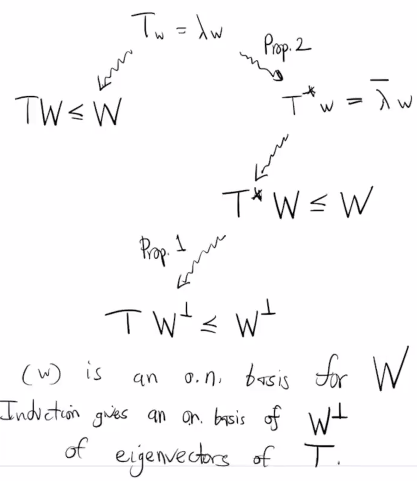
\includegraphics[width=0.25\textwidth]{Image 1122020.PNG}
    \end{center}
\end{proof}
\section{November 4, 2020}
Last time we talked about the spectral theorem.
\begin{definition}
A quadratic form is a homogeneous quadratic polynomial on $n$ variables. This equates to $\sum a_{ii}x_i^2+2\sum_{i<j}a_{ij}x_ix_j=\sum=x^tAx$ where $A$ is symmetric.
\end{definition}
Performing orthogonal coordinate changes, $x=Px$ where $P$ is in $O_n$. This changes $A$ to $P^tAP$. By the spectral theorem for real symmetric matrices, we can make $A$ a diagonal matrix with entries in $\R$. This is equal to $\lambda_1x_1^2+...+\lambda_nx_n^2$.

\subsection{Plane curves of degree 2}
$a_11x_1^2+2a_{12}x_1x_2+a_22X_2^2+B_1x_1+b_2x_2+c=0\iff x^tAx+Bx+c=0$.
\begin{theorem}
Every possibility is congruent to one of the examples (up to some isometry).
\end{theorem}
\begin{proof}
Given $x^tAx+Bx+c=0$. WLOG $A=\begin{pmatrix}
a&\\&b
\end{pmatrix}$. Then we get $ax_1^2+bx_2^2+b_1x_1+b_2x_2+c=0$

Case 1: $a,b\neq 0$. Complete the square. Substitute $x_1=x_1'-r$ for some $r\in \R$ to eliminate the $b_1x_1$ term. $r=\frac{b_1}{2a}$ works. Same for $x_2$. Get $ax_1^2+bx_2^2-c=0$.

Case 1a: $c\neq 0$. Divide equation by $c$. Get an ellipse or hyperbola

Case 1b: $c=0$. Get a point or two intersecting lines.

Case 2: $a\neq 0$, $b=0$. "Left as an exercise to the reader."

\end{proof}
\subsection{Quadric surfaces on on 3d space}
A similar analysis leads to $q(x_1,x_2,x_3)=1$, $x_3=Q(x_1,x_2)$, and some degenerate cases.

Now, look at skew-symmetric forms. Let $F$ be a field of characteristic not 2. $V$ an $F$-vector space. $<,>:V\times V\ra F$ a bilinear form.
\begin{proposition}
$<x,y>=-<y,x>$ for all $x,y \iff <x,x>=0$ for all $x$.
\end{proposition}
\begin{proof}
Left to right is easy because $<x,x>=-<x,x>$. This is where we use that the characteristic of the field is not 2.

Right to Left. If $<x,x>=0$ for all $x$ then $0=<x+y,x+y>=<x,x>+<x,y>+<y,x>+<y,y>\implies <x,y>=-<y,x>$
\end{proof}
\section{November 6, 2020}
$F$ is a field, $V$ is an $F$-vector space. $<,>:V\times V\ra F$ is a bilinear form. If the characteristic of $F$ is not 2 (nontrivial field), then the following conditions are equivalent: $<x,y>=-<y,x>$ for all $x,y\in V$, $<x,x>=0$ for all $x\in V$. If the characteristic of $F$ is 2, the alternating condition is more restrictive, and it is the better notion.
\begin{example}
On $F^2$, the determinant form is $<\begin{pmatrix}x_1\\x_2\end{pmatrix},\begin{pmatrix}y_1\\y_2\end{pmatrix}>=\det\begin{pmatrix}x_1&y_1\\x_2&y_2\end{pmatrix}=\mathbf{x}^t\begin{pmatrix}&1\\-1&\end{pmatrix}\mathbf{y}=1$ is alternating.
\end{example}
Recall that a real vector space $V$ with a symmetric bilinear form $<,>$ has an orthogonal basis. (Same for a complex vector space with a Hermitian form.) If in addition $<,>$ is positive definite, then $<,>$ has an orthonormal basis.

Alternating always implies symmetric.
\begin{theorem}
Let $<,>$ be nondegenerate, alternating form on $V$. A nondegenerate alternating form is also called symplectic. Then there exists a basis $(v_1,w_1,v_2,w_2,...,v_n,w_n)$ such that $<v_i,w_i>=1$, $<w_i,v_i>=-1$ and all other pairings of basis vectors give 0.
\end{theorem}
\begin{remark}
Put the images that I saved about conic sections into the previous day's section.
\end{remark}
\begin{theorem}[Matrix form of the previous theorem]
Let $A\in GL_m(F)$. Then $A^t=-A$ and zeros on diagonal. Then there exists $p\in GL_n(F)$ such that $P^tAP$ is a matrix with blocks of the form $\begin{pmatrix}&1\\-1&\end{pmatrix}$ along the diagonal and zeros everywhere else.
\end{theorem}
\begin{proof}
Induction on $\dim v$. If $\dim V=0$, we're done. Otherwise choose $v_1,w_1$ with $<v_1,w_1>\neq 0$. These exist since $<,>$ is nonnegative. Without loss of generality, let $<v_1,w_1>=1$ (scale $w_1$). Since $<v_1,v_1>=0$ so $w_1\notin \Span(v_1)$. Let $W=\Span(v_1,w_1)$ and $<,>$ is nondegenerate on $W$ since its matrix is $\begin{pmatrix}0&1\\-1&0\end{pmatrix}$, which is invertible. So, just as for symmetric forms, $V=W\oplus W^\perp$. The basis of $W$ is $(v_1,w_1)$ and the basis of $W^\perp$ is $(v_1,w_2,...,v_n,w_n)
$ of $W^\perp$ from inductive hypothesis.
\end{proof}
Also, skew-Hermitian forms. We're on to the LAST CHAPTER.
\begin{definition}
A \vocab{linear group} is a subgroup of $GL_n(\R)$ or $GL_n(\C)$ for some $n$.
\end{definition}
\begin{example}
$GL_n=GL_n(\R)$ and $O_n=\{P\in GL_n(\R):P^tP=I\}$. What do its elements preserve? Matrices of $O_n$ preserve dot product, length. Define $I_{3,1}=\begin{pmatrix}1&&&\\&1&&\\&&1&\\&&&-1\end{pmatrix}$. The Lorentz group is $O_{3,1}=\{P\in GL_n(\R):P^tI_{3,1}P=I_{3,1}\}.$ You get one of these gruops for every signature $(p,q)$. The unitary group $U_n=\{P\in GL_n(\C):P^*P=I\}$. The symplectic group $SP_{2n}=\{P\in GL_n(\R):P^tSP=S$ where $S=\begin{pmatrix}0&I\\I&1\end{pmatrix}$. "Things that preserve the standard symplectic form. Special linear group $SL_n=\{P\in GL_n(\R): \det P=1\}$ "preserves volume, up to a sign". Special orthogonal group $SO_n=O_n\cap SL_n$. You get a bunch of other groups, special lorentz group, special unitary, which are just $SL_n\cap O_{3,1}$ and $SL_n\cap U_n$ respectively. Note that $SSp_{2n}\cap SL_n=SSp_{2n}$.
\end{example}
\begin{example}[The General Orthogonal Group]
$GO_n=\{P\in GL_n(\R):\exists \lambda\in \R^\times s.t. P^tP=\lambda I$. Again, we get a series of other matrices $GU_n=\{P\in GL_n(\C):\exists \lambda\in \R^\times s.t. P^*P=\lambda I\}$ and $GSp_{2n}=\{P\in GL_n(\R):\exists \lambda\in\R^\times s.t. P^tSP=\lambda S\}$. Again, we can get an even wider variety of linear groups by looking at the matrices over the complex numbers.
\end{example}

Each of these groups has a geometry.
\begin{example}
$GL_n(\R)$ is an open subset of $\R^{n\times n}\cong \R^{n^2}$ since it's the inverse image under $\det:\R^{n\times n}\ra\R$ of the open subset $\R^\times \subset \R$. The inverse image under a continuous map of an open subset is open and we know that the determinant map is continuous since it's a polynomial. We'll say therefore that $\dim GL_n(\R)=n^2$. We can pick almost any $n^2$ elements in the matrix (with some constraints).
\end{example}
\begin{example}
The following are isomorphic: $\R/\Z$, $\R/2\pi\Z$, $U_1=\{z\in\C:z\overline{z}=1\},SO_2$. Geomtrically, the're all a circle.
\end{example}
\begin{example}
$SU_2$ is homeomorphic to a 3 dimensional sphere $S^3$. There are continuous maps $SU_2\ra S^3$ and $S^3\ra SU_2$ whose composition in either order is the identity map.
\end{example}
\section{November 8, 2020}
\begin{proposition}
$SU_2=\{\begin{pmatrix}
a & b \\
-\bar{b} & \bar{a}
\end{pmatrix}:a,b\in\C, \bar{a}a+\bar{b}b=1\}$.
\end{proposition}
\begin{proof}
Let $P\in \C^{2\times 2}$. Then $P\in SU_2 \iff P^*P=I$ and $\det P=1\iff P^*=P^{-1}$ and $ad-bc=1\iff \begin{pmatrix}
\bar{a} & \bar{c} \\
\bar{b} & \bar{d}
\end{pmatrix}=\begin{pmatrix}
d&-b\\
-c&a
\end{pmatrix}$ and $ad-bc=1\iff d=\bar{a},c=\bar b$
\end{proof}
\begin{corollary}
$SU_2=\left\{x_0\begin{pmatrix}
1&\\
&1
\end{pmatrix}+x_1\begin{pmatrix}
i&\\&-i\\
\end{pmatrix}+x_2\begin{pmatrix}
&1\\-1&
\end{pmatrix}+x_3\begin{pmatrix}
&i\\i&
\end{pmatrix}:x_0,...,x_3\in\R, x_0^2+x_2^2+x_3^2=1\right\}$
is the unit 3-sphere in the quaternion algebra. The quaternion algebra $\HH$ satisfies the above rules but no restriction on $x_0^2+x_1^2+x_2^2+x_3^2$.
\end{corollary}
\begin{fact}
$\HH$ satisfies all the axioms of a field except that multiplication is not commutative. $i^2=j^2=k^2=-1$, $ij=k, ji=-k$, ... We can represent this as a chain $i\ra j\ra k \ra i$.
\end{fact}
\begin{definition}
$\Q_8$ is a subgroup of $SU_2$ called the quaternion group of order 8.
\end{definition}
\begin{fact}
The eigenvalues of $P$ are $\{\lambda,\overline{\lambda}\}$ for some $\lambda\in\C$ with $|\lambda|=1$
\end{fact}
\begin{proof}
Since its unitary, |eigenvalues|=1, the product of the eigenvalues is $\det P=1$
\end{proof}
\begin{fact}
The characteristic polynomial of $P$ is $t^2-2x_0t+1$ with $-1\leq x_0\leq 1$
\end{fact}
\begin{proof}
$\tr P=2x_0$ and $\det P=1$
\end{proof}
\begin{fact}
$P$ is conjugate in $SU_2$ to $\begin{pmatrix}
\lambda&\\&\bar{\lambda}
\end{pmatrix}$
\end{fact}
\begin{proof}
$P$ is unitary so the spectral theorem says there exists $Q\in U_2$ such that $Q^{-1}PQ=\begin{pmatrix}
\lambda&\\&\bar{\lambda}
\end{pmatrix}$. Replace $Q$ by $\alpha$ where $\det(\alpha Q)=1=\alpha^2\det(Q)$.
\end{proof}
\begin{fact}
$P$ and $P'$ are conjugate in $SU_2$ if and only if $\tr P=\tr P'\iff P,P' $ have the same $x_0$-value
\end{fact}
The center of $SU_2$ is $\{\pm I\}$.

If $W\leq \HH$ is a 2 dimensional subspace containing 1,  choose an orthonormal basis 1, v. Then $v\in E$ so $v^2=-1$. $W=\{a1+bv:a,b\in\R\}$ is a copy of $\C$. You get all of these copies of the complex numbers. What happens when we intersect this with $SU_2$. $W\cap SU_2$ is teh unit circle in that $\C$.

\section{November 13, 2020}

Let $V=\Span(\mathbf i, \mathbf j,\mathbf k)\cong \R^3$. If $u,v\in V$ then $uv=(u_1i+u_2j+u_3k)(v_1i+v_2j+v_3k)=(-u\cdot v)+(u\times v)$ so $u\cdot v=-\frac{1}{2}\tr(uv)$. To make sense of this, the $(-u\cdot v)$ part is the real part and the $(u\times v)$ part is the $\mathbf i,\mathbf j,\mathbf k$ part, (nonreal part). For $P\in SU_2$, define "conjugation by $P$" by $x\mapsto PxP^{-1}$. Elements of the quaternions are just matrices. This map preserves trace so it restricts to a map $\gamma_p:V\ra V$, $x\mapsto PxP^{-1}$. Geometrically what is this map?
\begin{theorem}
$\gamma_p\in SO_3$. More specifically, I can tell you which rotation it is. If $P=\cos\theta+\sin\theta v$ where $v\in E$, then $\gamma_p$ is a rotation by $2\theta$ about the pole $v$.

$SU_2\ra SO_3$ is a surjective homomorphism with kernel $\{\pm I\}$ under the map $P\mapsto \gamma_p$.
\end{theorem}
\begin{proof}
Since $v$ is conjugate to $\mathbf i$ (both are in the conjugacy class $E$) by symmetry, we can reduce to the case where $v=\mathbf i$ so $P=\cos\theta+\sin\theta\mathbf i$. Then $\gamma_p(\mathbf i)=P\mathbf i P^{-1}=\mathbf i$, $\gamma_p(\mathbf j)=P\mathbf j P^{-1}\cos(2\theta)\mathbf j +\sin(2\theta)\mathbf k$, $\gamma_p(\mathbf k)=PkP^{-1}=-\sin(2\theta)\mathbf j +\cos(2\theta)\mathbf k$

Every element of $SO_3$ is a rotation of the previous type so $SU_2\ra SO_3$ is surjective. Also $\gamma_p=I\iff 2\theta\in 2\pi \Z\iff P=\pm I$.
\end{proof}
\begin{corollary}
$SO_3\cong \{\textrm{cosets of }\{\pm I\}\textrm{ in }SU_2\cong S^3/\sim$. This is the projective 3-space.
\end{corollary}
\subsection{Differential Equations and the Matrix Exponential}
Fix $a\in\C$. The function $x(t)=e^{at}$ for all $t\in\R$ is the unique solution to
\begin{equation*}
    \begin{split}
        \frac{dx}{dt}=ax\\
        x(0)=1
    \end{split}
\end{equation*}
Here are two ways to construct this function:
\begin{enumerate}
    \item Invoke the general existence and uniqueness theorem for linear ordinary differential equations
    \item Proe that $1+at+\frac{(at)^2}{2!}+\frac{(at)^3}{e!}$ converges to a differentiable function satisfying the above equations.
\end{enumerate}
\begin{example}
$a=i$. The $e^{it}=\cos t+i\sin t$ because the right hand side satisfies the differential equation.
\end{example}
\begin{definition}
Let $A\in\C^{n\times n}$. Then $e^A=I+A+\frac{A^2}{2!}+\frac{A^3}{3!}+...$. Then $e^{tA}$ is defined. We need to check that this converges for every $t\in\R$, it is differentiable, $\frac{d}{dt}e^{tA}=Ae^{tA}$, $e^0=I$.
\end{definition}
In general, suppose $u_1(t),u_2(t),...$ are functions $I\ra \R$. Define $||A||=\max_{i,j} a_{ij}$.
Wishful thinking:
\begin{enumerate}
    \item $$\sum_k u_k(t)$$ converges.
    \item If each $u_k$ is continuous then $u(t)=\sum_k u_k(t)$ is continuous
    \item If each $u_k$ is differentiable then $u$ is differentiable and $u'(t)=\sum_k u_k'(t)$.
\end{enumerate}
Then use the Weierstrass M-test here.
\section{November 16, 2020}
Some theorems from last time
The Weierstrass $M$-test. $\sum_k u_k(t)$ converges uniformly to a function $u:I\ra V$ if there exists real numbers $M_k$ such that $|u_k(t)|\leq M_k$ for all $t\in I$ and $\sum M_k<\infty$

If each $u_k$ is continuous and $\sum u_k(t)$ converges uniformly then $\sum u_k(t)$ is continuous.

If each $u_k$ is differentiable and $\sum u_k(t)$ converges and $\sum u'_k(t)$ converges uniformly then $\sum u_k(t)$ is differentiable and its derivative is $\sum u_k'(t)$.

Today, we're going to talk about the matrix exponential function $e^{tA}$ for $A\in \C^{n\times n}$. For $A\in \C^{n\times n}$, define $||A||=\max_{i,j}|a_{ij}|$. By induction on $k$, we have $||A^k||\leq n^{k-1}||A||^k$. Let $I=(-r,r)$. Let $V=\C^{n\times n}$. To define $e^{tA}$, we want to sum $u_k(t)=\frac{(tA)^k}{k!}$ which has $u_k'(t)==\frac{t^{k-1}A^k}{(k-1)!}$. These are bounded on $(-r,r)$ by $M_k=\frac{r^kn^{k-1}||A||^k}{k!}$ and $N_k=\frac{r^{k-1}n^{k-1}||A||^k}{(k-1)!}$. Then $\sum u_k(t)$ converges uniformly on $(-r,r)$ since $\sum M_k<\infty$ by the ratio test and also $\sum u_k'(t)$ converges uniformly on $(-r,r)$ since $\sum N_k<\infty$ also by the ratio test.

We conclude that $e^{tA}$ converges uniformly on $(-r,r)$ and $\frac{d}{dt}e^{tA}=Ae^{tA}$ at least for $t\in (-r,r)$.

Some properties of $e^{tA}$
\begin{enumerate}
    \item $\frac{d}{dt}e^{tA}=Ae^{tA}$
    \item $e^0=I$
    \item If $AB=BA$ then $e^Ae^B=e^{A+B}$
    \item $e^A$ is invertible with inverse $e^{-A}$
    \item If $B=PAP^{-1}$ then $e^B=Pe^AP^{-1}$
    \item If $A=\begin{pmatrix}
    \lambda_1&&\\&...&\\&&\lambda_n
    \end{pmatrix}$ then $e^A=A=\begin{pmatrix}
    e^\lambda_1&&\\&...&\\&&e^\lambda_n
    \end{pmatrix}$
\end{enumerate}
\begin{proof}[Proof of the second]
If $AB=BA$ then the binomial theorem applies $(A+B)^m=\sum_{k+l=m}\frac{m!}{k!l!}A^kB^l$ so $e^{A+B}=\sum_{m\geq 0}\frac{(A+B)^m}{m!}=\sum_{m\geq 0}\sum_{k+l=m}\frac{1}{m!}\frac{m!}{k!l!}A^kB^l=\sum_{k\geq 0}\sum_{l\geq 0}\frac{A^k}{k!}\frac{B^l}{l!}=e^Ae^B$. Rearranging terms is ok because everything converges absolutely.
\end{proof}
\begin{corollary}
For each $A\in\C^{n\times n}$ $\R\ra GL_n(\C)$, $t\mapsto e^{tA}$ is a homomorphism.
\end{corollary}
\begin{proof}
$e^{(t+u)A}=e^{tA+uA}=e^{tA}e^{uA}$ since $tA$ and $uA$ commute.
\end{proof}
\begin{definition}[One-parameter group]
A one-parameter group in $GL_n(\C)$ is a differentiable homomorphism from $\R$ to $GL_n(\C)$.
\end{definition}
Challenge: continuous homomorphisms from $\R$ to $GL_n(\C)$ are automatically differentiable.
\begin{proposition}
There is a bijection $\C^{n\times n}\ra $ one-parameter groups in $GL_n(\C)$, $A\mapsto (t\mapsto e^{tA}$, $\phi\mapsto \phi'(0)$.
\end{proposition}
\begin{proof}
We already showed that for each $A$, $t\mapsto e^{tA}$ is a one-parameter group. Suppose that $\phi:\R\ra GL_n(\C)$ is any one-parameter group. Let $A=\phi'(0)$. Let $A=\phi'(0)$. We want to show that $\phi(t)=e^{tA}$ for all $t\in \R$. We'll do this by showing that $\phi(t)$ satisfies the same differential equation and initial conditions as $e^{tA}$. We know that $\phi(s+t)=\phi(s)\phi(t)$. Take the derivative of this w.r.t. $s$. We get $\phi'(s+t)=\phi'(s)\phi(t)$. Evaluate at $s=0$ to get $\phi'(t)=A\phi(t)$. Also, $\phi(0)=A$.
\end{proof}
\begin{example}
Let $A=\mathbf i=\begin{pmatrix}
i&\\&-i
\end{pmatrix}$. Then $e^{tA}=\begin{pmatrix}
e^{it}&\\&e^{-it}
\end{pmatrix}\in SU_2$. This is going to be one of the longitudes.
\end{example}
For which $A\in \C^{n\times n}$ does the one-parameter group $t\mapsto e^{tA}$ land in $GL_n(\R)$? We claim that $A\in \R^{n\times n}\iff e^{tA}\in GL_n(\R)$ for all $t\in \R$.
\begin{proof}
By definition of $e^{tA}$, $e^{tA}\in GL_n(\R)$ when $A\in \R^{n\times n}$. Conversely, if $e^{tA}\in GL_n(\R)$ for all $t$, taking the derivative at $t=0$ gives $A\in \R$.
\end{proof}
For which $A\in GL_n(\C)$ is $e^{tA}\in U_n$ for all $t\in \R$? We claim that this is true if and only if $A$ is skew-Hermitian.
In general, $(e^A)^*=e^{A^*}=e^{-A}=(e^A)^{-1}$. Conversely, if $e^{tA}\in U_n$ for all $t\in \R$ then $(e^{tA})^*=(e^{tA})^{-1}\implies e^{tA^*}=e^{-tA}\implies A^*=-A$ after taking the derivative and evaluating at $t=0$.
\section{November 18, 2020}
For which $A$ is $e^{tA}$ in $O_n$ for all $t\in \R$?
Since $O_n=GL_n(\R)\cap U_n$, we need $A\in \R^{n\times n}$ and $A^*=-A$ or $A^t=-A$. This is equivalent to $A$ being a skew-symmetric matrix.
\begin{lemma}
For any $A\in \C^{n\times n}$, $\det e^A=e^{\tr A}$.
\end{lemma}
\begin{proof}
Conjugating $A$ by $P$ conjugates $e^A$ by $P$ so it doesn't change $e^A$. It also doesn't change $\tr(A)$. Therefore, WLOG, let $A$ be in Jordan canonical form.
Then
$$e^A=\begin{pmatrix}
e^{\lambda_1}&*&\\&...&\\&&e^{\lambda_n}
\end{pmatrix}
$$ so $\det e^A=e^{\tr A}$
\end{proof}
For which $A\in\R^{n\times n}$ is $e^{tA}\in SL_n(\R)$ for all $t\in \R$? The $A$ such that $\tr A=0$.
\begin{proof}
For $A\in \R^{n\times n}$, $\tr tA=0$ for all $t\in \R$ so $e^{\tr tA}=1$ so $e^{tA}\in SL_n(\R)$.
\end{proof}
\begin{definition}
$A$ is a $d$-dimensional manifold is a topologicla space $M$ such that every point $m\in M$ has an open neighborhood in $M$ that is homeomorphic to an open subset of $\R^d$.
\end{definition}
\begin{example}
A circle is a 1-dimensional manifold.
\end{example}
When can you solve for $y$ as a function of $x$ in the equation $ax+by+c=0$? That is, when does this equation describe the graph of a function. All we need is that $b\neq 0$. In other words, we need $\frac{\partial f}{\partial y}\neq 0$
\begin{theorem}[Implicit Function Theorem]
Suppose we are given the following:
\begin{enumerate}
    \item A system of equations $f(x,y)=0$ where $x=(x_1,...,x_m)$ and $y=(y_1,...,y_r)$ and $f=(f_1,...,f_r)$ and $f:U\ra \R^r$ is a $C^1$ function.
    \item A point $u\in Z(f)$ ($Z(f)$ is the set of solutions to $f=0$).
\end{enumerate}
If $\frac{\partial f}{\partial y}(u)$ is invertible where $((\frac{\partial f_i}{\partial y_j})(u))\in \R^{n\times n}$ then $Z(f)$ is a graph near $u$. This is equivalent to saying that there is an open neighborhood $U'$ of $u\in U$ such that $Z(f)\cap U'$ is a graph of some $g$ for some $C^1$ function $g:V\ra\R^r$, $V\subseteq\R^m$.
\end{theorem}
\begin{example}
Let's prove that $S^2=Z(x^2+y^2+z^2-1)$ in $\R^3$ is a manifold. We need to check each point $u\in S^2$. At $u$, not all of $x,y,z$ can be 0. WLOG $z\neq 0$ at $u$. Try to solve for $z$:$\frac{\partial f}{\partial z}=2z$ is nonzero at $u$, so the implicit function theorem says some neighborhood of $u$ in $S^2$ is the graph of a function $g(x,y)$. Secretly, $g(x,y)=\sqrt{1-x^2-y^2}$ or $-\sqrt{1-x^2-y^2}$. We conclude that $S^2$ is a manifold
\end{example}
\section{November 20, 2020}
\begin{theorem}
Let $G$ be a closed subgroup of $GL_n(\R)$. Then $G$ is a manifold. In fact, $G$ is $Z(f)$ for some function $f$ and is satisfies the condition of the implicit function theorem at each point.
\end{theorem}
\begin{definition}
A \vocab{differentiable path} in $G\leq GL_n(\R)$ as above is a differentiable function $\phi: \mathcal I\ra G$ where $\mathcal I$ is an open interval. If $0\in \mathcal I$, we get the velocity vector $\phi'(0)\in\R^{n\times n}$ which is tangent to the path, hence tangent to $G$.
\end{definition}
\begin{definition}[The Lie Algebra of G]
Here are three ways to describe the Lie Algebra $Lie(G)$.
\begin{enumerate}
    \item It's the tangent space to $G$ at $I$. It's the set $\{\phi'(0):\phi$ is a differentiable path in $G\}$.
    \item It's $\{A\in\R^{n\times n}$: the one-parameter group $e^{tA}$ is contained in $G$.
    \item If $G$ is defined by a system of polynomial equations $f=0$ satisfying the implicit function theorem, the lie algebra is $\{A\in\R^{n\times n}:I+\eps A$ satisfies the system of equations where $\eps^2=0$.
\end{enumerate}
\end{definition}
\begin{proof}[Proof that 2. is equivalent to 1.]
Suppose $A\in S$ where $S$ is the set from 2. Then the one-parameter group $\phi(t)=e^{tA}$ is centered in $G$. Then $\phi'(0)\in T$ where $T$ is the set from 1.
\end{proof}
Here's an algebraic way to take a derivative. Work in $\R[\eps]$ where $\eps^2=0$. If $f(x)=x^2+5x,$ then $f(x+\eps)=(x+\eps)^2+5(x+\eps)=(x^2+5x)+(2x+5)\eps$. We can then say that $f'$ is the $\eps$-component of $f$.
\begin{example}
Consider $O_n$. Then $Lie O_n=\{A\in\R^{n\times n}:(I+\eps A)^t(I+\eps A)=I\}$. This is equivalent to $I+\eps A^t+\eps A=I$ or $A^t+A=0$.
\end{example}
\begin{example}
Consider $SL_2$. The equation that defines $SL_2$ is $\det=1$. Thus TFAE, $A\in Lie SL_2$. Then $\det(I+\eps A)=1$ so $\tr A=0$.
\end{example}
Some properties of $Lie G$:
\begin{itemize}
    \item $Lie G$ is a vector space.
    \item If $A,B\in Lie G$, then $AB-BA\in Lie G$.
\end{itemize}
\begin{proof}
Use $\R[\eps,\eps']$ with $\eps^2=(\eps')^2=0$. If $A,B\in Lie G$ then $I+\eps A$, $I+\eps'B$ satisfy the equations of $G$ and then so does their commutator $(I+\eps A)(I+\eps'B)(I+\eps A)^{-1}(I+\eps' B)^{-1}=I+(AB-BA)\eps\eps'$.
\end{proof}
\begin{definition}[The Bracket]
Let $A,B\in Lie G$. Then $[A,B]=AB-BA$. This measures noncommutativity in some infinitesimal sense.
\end{definition}
\section{November 30, 2020}
Let $G$ be a closed subgroup of $GL_n(\R)$ or $GL_n(\C)$. Then $G$ is a manifold. It is the zero of some function $f$ satisfying the conditions of the implicit function theorem at each point. The \vocab{Lie algebra} can be described in three ways:
\begin{enumerate}
    \item The tangent space to $G$ at $I$. $Lie G=\{\phi'(0):\phi\textrm{ is a differentiable path in }G\textrm{ with }\phi(0)=I\}$
    \item $\{A\in\R^{n\times n}:\textrm{ the one-parameter group }e^{tA}\textrm{ is contained in }G\}$
    \item $\{A\in\R^{n\times n}:f(I+\eps A)=0\}$ assuming that $f$ is a tuple of polynomials in the matrix entries. Here we're working in $GL_n(\R)[\eps]$ where $\eps^2=0$.
\end{enumerate}
Some properties of $Lie G$ are that $Lie G$ is a vector space, the dimension of $Lie G$ is $\dim G$, if $A,B\in Lie G$ then $AB-BA\in Lie G$.
\begin{definition}
The \vocab{bracket} of two matrices is $[A,B]=AB-BA$.
\end{definition}
If $G$ is abelian then all matrices $A,B\in Lie G$ satisfy $[A,B]=0$.
\begin{definition}
A \vocab{Lie algebra} is a vector space $V$ equipped with a binary operation $[,]:V\times V\ra V$ such that
\begin{itemize}
    \item bilinearity
    \item $[A,A]=0$ ($\iff [B,A]=-[A,B]$)
    \item The Jacobi Identity $[A,[B,C]]+[B,[C,A]]+[C,[A,B]]=0$ for all $A,B,C$.
\end{itemize}
\end{definition}
Given $g\in G$, the translation map $G\ra G$, $x\mapsto gx$. This map is usually not a homomorphism, but it is a homeomorphism and it sends 1 to $g$.
\begin{example}
By definition, $G$ is a $d$-dimensional manifold if and only if every $g\in G$ has an open neighborhood homeomorphic to an open subset of $\R^d$. By homogeneity, it's enough to check this for $g=1$.
\end{example}
\begin{fact}
Any closed subgroup $G\subseteq GL_n(\R)$ is a manifold of the same dimension as its Lie algebra $\mathfrak g$.
\end{fact}
\begin{proof}[Idea of Proof]
$e:\R^{n\times n}\ra GL_n(\R),\, A\mapsto e^A$. It maps small neighbborhood of 0 to small neighborhood of $I$ under a homeomorphism. It restricts to a differentiable map $\mathfrak g\ra G$, $A\mapsto e^A$. It sends small neiborhoods of 0 in $\mathfrak g$ to small neighborhoods of $I$ in $G$.
\end{proof}
\begin{proposition}
If $H$ is an open subgroup of a linear group $G$ then it is closed in $G$.
\end{proposition}
\begin{proof}
$G$ consists of $H$ and all its cosets. $H$ is open. $G$ is the disjoint union of all the cosets, all of which have to be open. Take the union of all cosets of $H$ except for itself. This is open. Take the set difference of this union and $G$. This is closed because it's the complement of an open set and it is equal to $H$. Thus $H$ is closed. Note that the converse doesn't work since the infinite union of closed sets isn't necessarily closed. The converse works if we can also guarantee that $[G:H]$ is finite.
\end{proof}
\begin{example}
Let $G=\R^\times $ and $H=\R_{>0}$
\end{example}
\begin{definition}
$G$ is \vocab{path connected} if for every $x,y\in G$ there exists a continuous map $\phi:[0,1]\ra G$ with $\phi(0)=x$, $\phi(1)=y$.
\end{definition}
\begin{fact}
If $G$ is path connected, then $G$ is not a disjoing union of two nonempty open subsets.
\end{fact}
\begin{proposition}
Let $G$ be a path-connected linear group. Any nonempty open subset $U$ of $G$ generates the whole group $G$.
\end{proposition}
\begin{proof}
Let $H$ be the subgroup generated by $U$. We need to prove $H=G$. Choose $g\in U$. Then $g^{-1}U$ is an open neighborhood of $I$ and is contained in $H$. For each $h\in H$, $hg^{-1}U$ is an open neighborhood of $h$ in $G$ and is contained in $H$. Thus $H$ is open. $G$ is a disjoint union of open cosets. Since $G$ is path connected, all cosets of $H$ must be the same thing, or equivalently $H=G$.
\end{proof}
Remember that $G$ is simple if and only if $G\neq \{1\}$ and the only normal subgroup are itself and $\{1\}$.
\begin{theorem}
Is $SU_2$ is not simple because the center is normal. Its only normal subgroups are $\{I\}$ and $\{\pm I\}$.
\end{theorem}
\begin{proof}
Let $N$ be a normal subgroup of $SU_2$. Suppose that $N$ is not $\{I\}$ or $\{\pm I\}$, so $N$ contains some $g\neq I$. Since $N$ is normal, $N$ contains the conjugacy class of $g$, a lattitude $\Lambda$. Then $I\in g^{-1}\Lambda \subseteq N$. $N$ contains all these lattitudes too so $N$ contains an open neighborhood of $I$. By the previous proposition, $N=SU_2$.
\end{proof}
\section{December 2, 2020}
\begin{corollary}
$SO_3$ is simple.
\end{corollary}
\begin{proof}
We have $\gamma: SU_2\ra SO_3$ with kernel $\{\pm I\}$. The correspondence theorem says there is a bijection between the normal subgroups of $SU_2$ and the normal subgroups of $SO_3$. $\{\pm I\}$ is the only normal subgroup in $SU_2$ and it gets mapped to the trivial group in $SO_3$.
\end{proof}
\begin{theorem}
Let $F$ be a field with $|F|\geq 4$. Then the only normal subgroups of $SL_2(F)$ are $\{I\}$, $\{\pm\},$ and $SL_2(F)$. If the characteristic of $F$ is 2, then $-1=1$, $-I=I$, and $\{\pm I\}=\{I\}$. We'll prove it for $|F|$.

The square root lemma: For $a\in F$, the equation $x^2=a$ has less than or equal to 2 solutions. If $|F|>5$ then there exists $r\in F$ such that $r^2\neq \{0,1,-1\}$.

Suppose $N$ is a normal subgroup of $SL_2(F)$ and $N$ is not conatined in $\{\pm I\}$. We need to show that $N=SL_2(F)$. First, $N$ contains come matrix $B$ with distinct eigenvalues. Choose $N-\{\pm I\}$. Then $A$ is not a scalar times $I$. Choose $v_1$ such that $v_1$ is not an eigenvector of $A$. Let $v_2=Av_1$ so $(v_1,v_2)$ is a basis of $F^2$. Choose $r\in F$ such that $r^2\notin\{0,1,-1,\}$. Let $P\in GL_2$ be such that $Pv_1=rv_1$ and $Pv_2=r^{-1}v_2$. Then the determinant of $P$ is 1 so $P\in SL_2(F)$. Then $PAP^{-1},\, APA^{-1}P^{-1}\in N$. Call $B=APA^{-1}P^{-1}$. Then $APA^{-1}P^{-1}v_2=r^2v_2$. Thus $Bv^2=r^2v_2$. The eigenvalues of $B$ are $r^2$ and $r^{-2}$ since $\det B=1$. Since $r^2\notin\{0,1,-1,\}$ $B$ is not the zero, identity, or -identity matrix. Next, let $C$ be the setf of matrices in $SL_2(F)$ with eigenvalues $s,s^{-1}$. Then $C$ is a single conjugacy class of $SL_2(F)$. Let $S=\begin{pmatrix} s&\\&s^{-1}\end{pmatrix}$. Then conjugacy class of $S$ is a subset of $C$. We want to show the other inclusion now. Suppose that $Q\in C$. Then $Q$ has distinct eigenvalues so it is diagonalizable. It is conjugate to $S$ in $GL_2(F)$. We know that $Q=LSL^{-1}$ for some $L\in GL_2(F)$. Then
$$Q=L\begin{pmatrix}
a&\\&1
\end{pmatrix}S\begin{pmatrix}
a^{-1}&\\&1
\end{pmatrix}L^{-1}$$ for any $a\in F^\times=MSM^{-1}$. Choose $a=(\det L^{-1}$ so that $\det M=1$ so $M\in SL_2(F)$. So $Q$ is conjugate to $S$ in $SL_2(F)$. Next, we show that $\begin{pmatrix}
1&*\\&1
\end{pmatrix}\in N$ for all $x\in F$.
\end{theorem}
\begin{proof}
$\begin{pmatrix}
1&*\\&1
\end{pmatrix}=\begin{pmatrix}
s^{-1}&\\&s
\end{pmatrix}
\begin{pmatrix}
s&sx\\&s^{-1}
\end{pmatrix}\in N$. Next, we show that $\begin{pmatrix}
1&\\y&
\end{pmatrix}\in N$ for all $y\in F$. the proof is similar. Consequently, $N=SL_2$. The matrices in step 3 and 4 generate $SL_2(F)$. This somes from some old PSET :).
\end{proof}
Let $Z$ be the center of $SL_2(F)$. Then $\{\pm I\}\subseteq Z$ is a proper normal subgroup of $SL_2(F)$. So $Z=\{\pm I\}$
\begin{definition}
$PSL_2(F)=SL_2(F)/Z$
\end{definition}
\begin{corollary}
If $|F|\geq 4$, then $PSL_2(F)$ is simple. The proof follows from the correspondence theorem.
\end{corollary}
\begin{table}[h]
    \centering
    \begin{tabular}{c|c|c}
        q & $PSL_2(F)$ & simple? \\
        2 & $S_3$ & no \\
        3 & $A_4$ & no \\
        4 & $A_5$ & yes \\
        5 & $A_5$ & yes \\
        6 & & yes \\
        7 & & yes \\
        8 & & yes \\
        9 & $A_6$ & yes
    \end{tabular}
    \caption{Accidental Isomorphisms}
    \label{tab:my_label}
\end{table}
\section{December 4, 2020}
Classification of finite simple groups: every finite simple group is one of the following:
\begin{itemize}
    \item $C_p$ for some prime $p$
    \item $A_n$ for some $n\geq 5$
    \item $PSL_2(F_q)$ for some prime power $q\geq 4$
    \item One of 26 "sporadic" groups, the largest of which is called the Monster group
\end{itemize}
\begin{definition}
A sequence of homomorphisms
$$A\ra[\alpha]B\ra[\beta]C$$ is exact (at $B$) if $\im\alpha=\ker\beta$.
\end{definition}
\begin{example}
$$\R\ra[\alpha]\C^\times\ra[\beta]\R^\times$$
$$t\mapsto e^{it}\mapsto |e^{it}|$$
is exact, since $\im\alpha=\ker\beta$, the unit circle.
\end{example}
\begin{definition}
$$G_0\ra[\alpha_1]G_1\ra[\alpha_2]G_2\ra...\ra[\alpha_n]G_n$$
is exact if it is exact at each joint. $\im\alpha_1=\ker\alpha_{i+1}$.
\end{definition}
\begin{example}
The following are equivalent
\begin{itemize}
    \item $1\ra A\ra[\phi] B$ is exact
    \item $\ker\phi=1$
    \item $\phi$ is injective
\end{itemize}
\end{example}
\begin{example}
TFAE
\begin{itemize}
    \item $B\ra[\psi]C\ra 1$ is exact
    \item $\im\psi=C$
    \item $\psi$ is surjective
\end{itemize}
\end{example}
\begin{definition}
An exact sequence of the form $1\ra A\ra B\ra C\ra 1$ is called a short exact sequence.
\end{definition}
\begin{example}
If $\phi:B\ra C$ is a surjective homomorphism, then
$$1\ra\ker\phi\ra[i]B\ra[\phi]C\ra 1$$ is a short exact sequence.
\end{example}
\section{December 7, 2020}
\begin{definition}
$Aut(G)$ is the group of automorphisms of $G$.
\end{definition}
\begin{example}
$C_5$. For each integer $r$, there is a homomorphism $\alpha_r:C_5\ra C_5$, $g\mapsto g^r$. If $5|r$, then $g^r=1$ so $\alpha_r$ sends $C_5$ to 1 so $\alpha_r$ is not an automorphism. If $5\notdiv r$, then $g^r$ generates $C_5$ so $\alpha_r$ is an automorphism. Then $\alpha_r=\alpha_{r'}\iff g^r=g^{r'}\iff r\equiv r'(\mod{5})$. And $\alpha_r\circ \alpha_s=\alpha_{rs}$. We conclude that $C_5\cong (\Z/5Z)^\times$. There are 4 such automorphisms.
\end{example}
\begin{example}
Every finite abelian group is a product of cyclic groups. $C_p^n$ is a vector space of over the field $F_p$ of dimension $p$. $Aut(C_p^n)=GL_n(F_p)$.
\end{example}
\begin{definition}
A \vocab{complement of N in G} is a subgroup $H\leq G$ such that $NH=G$ and $N\cap H=1$.
\end{definition}
\begin{proposition}
If $H$ is a completement of $N$ which is a normal subgroup of $G$ then the map $N\times H\ra G$, $(x,h)\mapsto xh$ is a bijection of sets.
\end{proposition}
\begin{definition}
Given groups $N$ and $H$ and a homomorphism $H\ra Aut N$ and $h\mapsto \phi_h$, define $N\rtimes H$ to be the set $N\times H$ with the binary operation $(x,h)(x',h')=(x\phi_h(x'),hh')$.
\end{definition}
\begin{proposition}
$N\rtimes H$ is a group. It's called the semidirect product of $N$ and $H$ with respect to $\phi$. The proof is just a matter of checking the group axioms.
\end{proposition}
The group $N\rtimes H$ has two obvious subgroups: $\{(x,1):x\in N\}$ is a copy of $N$ in $N\rtimes H$ and $\{(1,h):h\in H\}$ is a copy of $H$. We get a short exact sequence: $1\ra N\ra N\rtimes H\ra H\ra 1$.
\begin{proposition}
If $H$ is a complement of $N$ which is a normal subgroup of $H$ then $H$ acts on $N$ by conjugation via $\phi:H\ra Aut N$, $h\mapsto (x\mapsto hxh^{-1}$ and $G\ra[\sim]N\rtimes H$, $(x,h)\mapsto xh$.
\end{proposition}
\begin{example}
Start with $C_n=N$. We have a homomorphism $\phi:\{\pm I\}\ra Aut C_n$, $1\mapsto (x\mapsto x)$, $-1\mapsto (x\mapsto x^{-1})$. We can form the semidirect product $C_n\rtimes \{\pm I\}$. What is it? $D_n$.
\end{example}
\begin{example}
$\R^n$ is a normal subgroup of the group of isometries. Thus $O_n$ acts on $\R^n$ under matrix-vector multiplication so $M_n\cong \R^n\rtimes O_n$.
\end{example}
\section{December 9, 2020}
Today, we're going to talk about tensor products. polyhedra and the Dehn invariant (time-permitting).
Let $V,W$ be $\R$-vector spaces. Given $v\in V$ and $w\in W$, can we multiply to get $v\otimes w$? Yes. In which vector space would $v\otimes w$ lie? $V\otimes W$. We define $\R^m\otimes \R^n=\R^{mn}$. This is not to be confused with $\R^3\oplus \R^2=\R^5$.

There is a unique way to extend the $\otimes$ on basis vectors to all vectors, to define $v\otimes w$ for all $v\in \R^3$, $w\in \R^2$ in such a way that $\R^2\times \R^3\ra \R^2\otimes \R^3$, $(v,w)\mapsto v\otimes w$ is a bilinear form. For example, if $v=2e_1+5e_3$ and $w=3f_1+7f_2$. Then $v\otimes w=6e_1\otimes f_1+14e_1\otimes f_2+15e_3\otimes f_1 + 35e_3\otimes f_2$.

Given $V$ and $W$, $\R$ vector spaces. How do we define $V\otimes W$?
Wrong: $G$ is an $\R$-vector space with one basis vector for each pair $(v,w)$ with $v\in V$ and $w\in W$, and define $v\otimes w$ is the basis vector $(v,w)$ of $G$. This makes $G$ infinite dimensional and $(v_1+v_2)\otimes w=v_1\otimes w+v_2\otimes w$ won't hold. The three vectors will all be different bases (and consequently linearly independent). This is a contradiction since there is an obvious linear dependency among the three elements. Let $\mathcal R$ be the subspace of $G$ spanned by
\begin{itemize}
    \item $(v_1+v_2,w)-(v_1,w)-(v_2,w)$
    \item $(cv,w)-c(v,w)$
    \item $(v,w_1+w_2)-(v,w_1)-(v,w_2)$
    \item $(v,cw)-c(v,w)$
\end{itemize}
for all $v_1,v_2\in V$ and $w\in W$ for all $c\in \R$, $v\in V$ and $w\in W$. Finally, define $V\otimes W=G/\mathcal R$. Then the things in $\mathcal R$ get identified to zero so it's bilinear and stuff.

The same construction works over any field $\mathbb F$. If $V$ and $W$ are $F-vector spaces$, then we can form $V\otimes W$.
\begin{example}
$\C\otimes\C$ is a 4-dimensional $\R$ vector space and $\C\otimes \C$ is a 1-dimensional $\C$-vector space. $\R$ is a $\Q$-vector space (under addition and scalar multiplication) of infinite dimension. $\sqrt2, \sqrt3,...,$ are $\Q$-linearly dependent. $\Q\pi$ is a 1-dimensional $\Q$-subspace of $\R$. $\R/\Q\pi$ is another infinite-dimensional vector space.
\end{example}
\subsection{The Dehn Invariant}
Suppose we have a polyhedron. Slice the polyhedra. Get all the pieces. Glue the pieces again and you get a new polyhedron. Suppose you called the polyedron you started with $P$ and the one you ended with $P'$. Obviously, the areas of $P$ and $P'$ will stay the same. There's another quantity that's preserved. Fix your attention on one of the edges of $P$. There is such thing as the dihedral angle. The angle between two faces that meet along an edge $e$. Call this angle $\theta_e$. Call the length of $e$ $l_e$. Then $$\sum_{e\textrm{ an edge}}l_e\otimes \theta_e\in\R\otimes \R/\Q\pi$$.
\begin{theorem}
Two polyhedra are scissor-congruent if and only if they have the same volume and have the same Dehn-invarant.
\end{theorem}
\begin{itemize}
    \item The regular tetrahedron has dihedral angles $\cos^{-1}(\frac{1}{3})\in\Q\pi$ and hence Dehn invariant
    $$\sum_{i=1}^61\otimes\cos^{-1}(\frac{1}{3})\neq 0$$ in $\R_\Q\otimes \R/\Q\pi$
    \item The cube has dihedral angles $\pi/2\in\Q\pi$ and hence the Dehn invariant 0.
\end{itemize}
Some non-regular tetrahedra have Dehn invariant 0. An open problem is to classify them all.
\end{document}
